%%%%%%%%%%%%%%%%%%%%%%%%%%%%%%%%%%%%%%%%%%%%%%%%%%%%%%%%%%%%%%%%%%%%%%%%%%%%%%%%
%2345678901234567890123456789012345678901234567890123456789012345678901234567890
%        1         2         3         4         5         6         7         8
\documentclass[journal]{IEEEtran}  % Comment this line out

\IEEEoverridecommandlockouts                       % This command is only
% needed if you want to
% use the \thanks command
% See the \addtolength command later in the file to balance the column lengths
% on the last page of the document



% The following packages can be found on http:\\www.ctan.org

%fixes to the latex2e kernel
%\usepackage{fixltx2e} %this is not needed after 2015
\usepackage{fix-cm}
\usepackage{etex}

%fix double floats numbering and positioning
\usepackage{dblfloatfix}

%checks for obsolete packages
\usepackage{nag}


%%% Local Variables: 
%%% mode: latex
%%% End: 

%Note: pagination needs to be loaded after graphics, because mdframed
%needs to be loaded after xcolor to keeep the our options for the latter
%colors
\makeatletter
\@ifpackageloaded{xcolor}{}{%
\usepackage[table,x11names,dvipsnames,svgnames]{xcolor}%
}
\makeatother

%colors in table
\usepackage{colortbl}

%pdf
\usepackage{graphicx}
\usepackage{wrapfig}

% Lyft colors (see https://design.lyft.com/re-approaching-color-9e604ba22c88)
\input{preamble/graphicsColors}

%%% Local Variables: 
%%% mode: latex
%%% End: 

\usepackage{cite}

%advanced typesetting
\usepackage{microtype}

%extensions for tables
\usepackage{array}
\usepackage{multirow}
\usepackage{booktabs}
\usepackage{makecell} %introduces \thead and \makecell

%compact paragraph title
\newcommand{\myparagraph}[1]{\textbf{\emph{#1}}.}
%\newcommand{\subparagraph}[1]{\emph{#1}.}

%provide options for changing spacing in enumeration environments
\ifcsname labelindent\endcsname
\let\labelindent\relax
\fi
\usepackage[inline]{enumitem}

%provides subfloats (subcaption replaces subfig and subfigure, but
%might not be compatible with some classes)
\usepackage{subfig}

\providecommand{\ie}{i.e.}
\providecommand{\eg}{e.g.}
\providecommand{\etal}{et al.}

%set more relaxed constraints on the floats
\setcounter{topnumber}{2}
\setcounter{bottomnumber}{2}
\setcounter{totalnumber}{4}
\renewcommand{\topfraction}{0.85}
\renewcommand{\bottomfraction}{0.85}
\renewcommand{\textfraction}{0.15}
\renewcommand{\floatpagefraction}{0.7}

%Make an enumeration with a letter+progressive number
\newenvironment{lenumerate}[2][]
{\begin{enumerate}[label=(#2\arabic*),leftmargin=0.2in,itemindent=0.15in,#1]}
{\end{enumerate}}

%Make an letter+progressive number description list
\newenvironment{ldescription}[2][]
{\begin{lenumerate}{#2}%
\let\bitem\item%
\renewcommand{\item}[1][]{\bitem\textsl{##1}:~}}
{\end{lenumerate}}


 %The following sets the labeling for inline enumerations

\setlist*[enumerate,1]{label={\itshape\arabic*)}}

%Define macro to make paragraph headings always end with a full stop
\makeatletter
\newcommand{\paragraphswithstop}{%
\let\copyparagraph\paragraph%
\renewcommand\paragraph[1]{\copyparagraph{##1.}}%
}
\makeatother

%Package to frame text in boxes
\usepackage[framemethod=tikz]{mdframed}

%%% Local Variables: 
%%% mode: latex
%%% End: 

%
% Allow easy definition of starred version of commands
% Ref: https://tex.stackexchange.com/questions/202504/macro-to-add-starred-version-of-command
\usepackage{suffix}

% Allow definition of environments with extra final code
\usepackage{environ}

% Insert a prefix-argument-postfix text only if argument is non-empty
% Needs to use a savebox to avoid evaluating the argument multiple times
\makeatletter
\newsavebox{\boxifnotempty}
\newcommand{\displayifnotempty}[3]{\sbox\boxifnotempty{#2}\setbox0=\hbox{\usebox{\boxifnotempty}\unskip}%
\ifdim\wd0=0pt
\else
 #1\usebox{\boxifnotempty}#3%
\fi%
}
\newcommand{\ifempty}[2]{\setbox0=\hbox{#1\unskip}%
\ifdim\wd0=0pt%
 #2%
\fi%
}
\newcommand{\ifnotempty}[2]{\setbox0=\hbox{#1\unskip}%
\ifdim\wd0>0pt%
 #2%
\fi%
}
\makeatother

%introduce the algorithmic environment and the algorithm floats
\usepackage{algpseudocode}
\usepackage{algorithm}

%macros for storing definitions across compilations
\usepackage{scrlfile}

\makeatletter
%mark a definition to be stored in the aux file
\newcommand*\newstoreddef[1]{
  \BeforeClosingMainAux{%
    \immediate\write\@auxout{%
      \string\restoredef{#1}{\csname #1\endcsname}%
    }%
  }%
}
%used by the aux file to restore the definition
\newcommand*{\restoredef}[2]{% used at the aux file
  \expandafter\gdef\csname stored@#1\endcsname{#2}%
}
%show the stored definition (user command to ask for the value)
\newcommand*{\storeddef}[1]{
  \@ifundefined{stored@#1}{0}{\csname stored@#1\endcsname}%
}
\makeatother

%Add values to non-counter definitions (works with non-integers)
\newcommand{\addtovar}[2]{\pgfmathparse{#1+#2}\xdef#1{\pgfmathresult}}
\newcommand{\zerovar}[1]{\xdef#1{0}}

%Insert content of a PGF variable 
\newcommand{\pgfprint}[1]{\pgfmathparse{#1}\pgfmathresult}

%Package to get PDF page numbers
\usepackage{pageslts}
%\pagenumbering{arabic}
%Output content of enviroment both to the document and to the log file
%In the log file, the content is marked by start/end delimiters, and
%macros are not expanded.
\NewEnviron{tee}{\BODY\typeout{Marker Tee [start] ^^J \BODY ^^JMaker Tee [end]}}


%%% Local Variables: 
%%% mode: latex
%%% End: 

%AMS typesetting
\makeatletter
\@ifpackageloaded{amsmath}{}{%
\usepackage[cmex10]{amsmath}%
}
\makeatother
\usepackage{mathtools}
\usepackage{amssymb,amsfonts}
\makeatletter
\@ifundefined{proof}{%
\usepackage{amsthm}%
}{}
\makeatother

\usepackage{mathtools}

%Common math statements environments
\makeatletter
\@ifundefined{theorem}{
\newtheorem{theorem}{Theorem}
\newtheorem{corollary}{Corollary}
\newtheorem{proposition}{Proposition}
\newtheorem{lemma}{Lemma}
\newtheorem{remark}{Remark}
\newtheorem{fact}{Fact}
}{}
  %SIAM article classes give their own Definition and Remark environments
\@ifundefined{definition}{
  \newtheorem{definition}{Definition}
}
% \@ifundefined{remark}{
%   \newtheorem{remark}{Remark}
% }
\makeatother
\newtheorem{problem}{Problem}
\newtheorem{assumption}{Assumption}
\newtheorem{property}{Property}
\newcommand{\rmss}[1]{_{\textrm{#1}}}

%%% Local Variables: 
%%% mode: latex
%%% End: 

%Spaces
\newcommand{\real}[1]{\mathbb{R}^{#1}{}}
\newcommand{\complex}[1]{\mathbb{C}^{#1}{}}
\newcommand{\naturals}[1]{\mathbb{N}^{#1}{}}
\newcommand{\integers}[1]{\mathbb{Z}^{#1}{}}
\newcommand{\sphere}[1]{{\mathbb{S}^{#1}}{}}
\newcommand{\stiefel}{\mathrm{St}}
\newcommand{\grassmann}{\mathrm{Grass}}
\newcommand{\GL}{\mathbb{GL}}

%short-hand for matrices
\newcommand{\bmat}[1]{\begin{bmatrix}#1\end{bmatrix}}
\newcommand{\Bmat}[1]{\begin{Bmatrix}#1\end{Bmatrix}}
\newcommand{\pmat}[1]{\begin{pmatrix}#1\end{pmatrix}}

%supertscript operators
\newcommand{\transpose}{^\mathrm{T}}
\newcommand{\hermitian}{^\mathrm{H}}
\newcommand{\inverse}{^{-1}}
\newcommand{\pinverse}{^\dagger}
\newcommand{\orth}{^{\bot}}
\newcommand{\apstar}{^{\ast}}

%parentheses-based operators
\newcommand{\cross}[1]{[#1]_{\times}\!}
\newcommand{\crossinv}[1]{[#1]_{\times}^{\textrm{inv}}\!}

%equality
\newcommand{\defeq}{\doteq}


%Norms, absolute values, and inner products
\DeclarePairedDelimiter{\abs}{\lvert}{\rvert}
\DeclarePairedDelimiter{\ceil}{\lceil}{\rceil}
\DeclarePairedDelimiter{\norm}{\lVert}{\rVert}
\newcommand{\frob}[1]{\norm{#1}_F}
\newcommand{\bigfrob}[1]{\bignorm{#1}_F}
\newcommand{\metric}[3][]{g_{#1}\left(#2, #3\right)}
\newcommand{\metrica}[3]{\langle #2, #3\rangle_{#1}}

%Derivatives
\newcommand{\de}{\mathrm{d}}
\newcommand{\dert}[1][]{\frac{\de #1}{\de t}}
\newcommand{\ddert}[1][]{\frac{\de^2 #1}{\de t^2}}
%Vector
\newcommand{\vct}[1]{\mathbf{#1}}
\newcommand{\pder}[2][]{\frac{\partial #1}{\partial #2}}
%named operators
\DeclareMathOperator*{\Land}{\bigwedge}
\DeclareMathOperator{\rank}{rank}
\DeclareMathOperator{\diag}{diag}
\DeclareMathOperator{\blkdiag}{blkdiag}
\DeclareMathOperator{\symm}{sym}
\DeclareMathOperator{\asym}{skew}
\DeclareMathOperator*{\argmin}{\arg\!\min}
\DeclareMathOperator{\softmin}{softmin}
\DeclareMathOperator*{\argmax}{\arg\!\max}
\DeclareMathOperator{\trace}{tr}
\DeclareMathOperator{\vecspan}{span}
\DeclareMathOperator{\vecnull}{null}
\DeclareMathOperator{\vecnullity}{nullity}
\DeclareMathOperator{\vecop}{vec}
\DeclareMathOperator{\stack}{stack}
\DeclareMathOperator{\hstack}{hstack}
\DeclareMathOperator{\vstack}{vstack}
\DeclareMathOperator{\sign}{sign}
\DeclareMathOperator{\sinc}{sinc}
\DeclareMathOperator{\expm}{expm}

\DeclareMathOperator{\grad}{{grad}}
\DeclareMathOperator{\D}{D\!}
\DeclareMathOperator{\Dgrad}{{Dgrad}}
\DeclareMathOperator{\hess}{{Hess}}

\DeclareMathOperator*{\inj}{inj}
\DeclareMathOperator{\hull}{hull}

\DeclareMathOperator{\proj}{{proj}}

\DeclareMathOperator*{\logm}{logm}
\DeclareMathOperator{\Log}{Log}
\DeclareMathOperator{\LogNorm}{\frac{Log}{\norm{Log}}}
\DeclareMathOperator{\DLog}{DLog}
\DeclareMathOperator{\DLogNorm}{D\frac{Log}{\norm{Log}}}

\DeclareMathOperator{\conv}{conv}
\DeclareMathOperator{\cvxhull}{co}

\DeclareMathOperator{\dist}{dist}

\DeclareMathOperator*{\bigO}{O}

%\DeclareMathOperator*{\Pr}
\newcommand{\intersect}{\cap}
\newcommand{\union}{\cup}
\DeclareMathOperator*{\Or}{\bigvee}

%text for constrained optimization
\newcommand{\subjectto}{\textrm{subject to }}

%%% Local Variables: 
%%% mode: latex
%%% End: 


%memberships
\newcommand{\iV}[1][]{{i \in V_{#1}}}
\newcommand{\ijE}[1][]{(i,j) \in E_{#1}}

%operators
\DeclareMathOperator{\dg}{{deg}}
\DeclareMathOperator{\diam}{{Diam}}

%%% Local Variables: 
%%% mode: latex
%%% End: 

% This file was generated by the scriptgenerateNotation
% Do not modify this file directly

% Shortand notation for vectors and their derivatives
\providecommand{\va}{\vct{a}}
\providecommand{\dva}{\dot{\vct{a}}}
\providecommand{\tva}{\tilde{\vct{a}}}
\providecommand{\dtva}{\dot{\tilde{\vct{a}}}}
\providecommand{\vb}{\vct{b}}
\providecommand{\dvb}{\dot{\vct{b}}}
\providecommand{\tvb}{\tilde{\vct{b}}}
\providecommand{\dtvb}{\dot{\tilde{\vct{b}}}}
\providecommand{\vc}{\vct{c}}
\providecommand{\dvc}{\dot{\vct{c}}}
\providecommand{\tvc}{\tilde{\vct{c}}}
\providecommand{\dtvc}{\dot{\tilde{\vct{c}}}}
\providecommand{\vd}{\vct{d}}
\providecommand{\dvd}{\dot{\vct{d}}}
\providecommand{\tvd}{\tilde{\vct{d}}}
\providecommand{\dtvd}{\dot{\tilde{\vct{d}}}}
\providecommand{\ve}{\vct{e}}
\providecommand{\dve}{\dot{\vct{e}}}
\providecommand{\tve}{\tilde{\vct{e}}}
\providecommand{\dtve}{\dot{\tilde{\vct{e}}}}
\providecommand{\vf}{\vct{f}}
\providecommand{\dvf}{\dot{\vct{f}}}
\providecommand{\tvf}{\tilde{\vct{f}}}
\providecommand{\dtvf}{\dot{\tilde{\vct{f}}}}
\providecommand{\vg}{\vct{g}}
\providecommand{\dvg}{\dot{\vct{g}}}
\providecommand{\tvg}{\tilde{\vct{g}}}
\providecommand{\dtvg}{\dot{\tilde{\vct{g}}}}
\providecommand{\vh}{\vct{h}}
\providecommand{\dvh}{\dot{\vct{h}}}
\providecommand{\tvh}{\tilde{\vct{h}}}
\providecommand{\dtvh}{\dot{\tilde{\vct{h}}}}
\providecommand{\vi}{\vct{i}}
\providecommand{\dvi}{\dot{\vct{i}}}
\providecommand{\tvi}{\tilde{\vct{i}}}
\providecommand{\dtvi}{\dot{\tilde{\vct{i}}}}
\providecommand{\vj}{\vct{j}}
\providecommand{\dvj}{\dot{\vct{j}}}
\providecommand{\tvj}{\tilde{\vct{j}}}
\providecommand{\dtvj}{\dot{\tilde{\vct{j}}}}
\providecommand{\vk}{\vct{k}}
\providecommand{\dvk}{\dot{\vct{k}}}
\providecommand{\tvk}{\tilde{\vct{k}}}
\providecommand{\dtvk}{\dot{\tilde{\vct{k}}}}
\providecommand{\vl}{\vct{l}}
\providecommand{\dvl}{\dot{\vct{l}}}
\providecommand{\tvl}{\tilde{\vct{l}}}
\providecommand{\dtvl}{\dot{\tilde{\vct{l}}}}
\providecommand{\vm}{\vct{m}}
\providecommand{\dvm}{\dot{\vct{m}}}
\providecommand{\tvm}{\tilde{\vct{m}}}
\providecommand{\dtvm}{\dot{\tilde{\vct{m}}}}
\providecommand{\vn}{\vct{n}}
\providecommand{\dvn}{\dot{\vct{n}}}
\providecommand{\tvn}{\tilde{\vct{n}}}
\providecommand{\dtvn}{\dot{\tilde{\vct{n}}}}
\providecommand{\vo}{\vct{o}}
\providecommand{\dvo}{\dot{\vct{o}}}
\providecommand{\tvo}{\tilde{\vct{o}}}
\providecommand{\dtvo}{\dot{\tilde{\vct{o}}}}
\providecommand{\vp}{\vct{p}}
\providecommand{\dvp}{\dot{\vct{p}}}
\providecommand{\tvp}{\tilde{\vct{p}}}
\providecommand{\dtvp}{\dot{\tilde{\vct{p}}}}
\providecommand{\vq}{\vct{q}}
\providecommand{\dvq}{\dot{\vct{q}}}
\providecommand{\tvq}{\tilde{\vct{q}}}
\providecommand{\dtvq}{\dot{\tilde{\vct{q}}}}
\providecommand{\vr}{\vct{r}}
\providecommand{\dvr}{\dot{\vct{r}}}
\providecommand{\tvr}{\tilde{\vct{r}}}
\providecommand{\dtvr}{\dot{\tilde{\vct{r}}}}
\providecommand{\vs}{\vct{s}}
\providecommand{\dvs}{\dot{\vct{s}}}
\providecommand{\tvs}{\tilde{\vct{s}}}
\providecommand{\dtvs}{\dot{\tilde{\vct{s}}}}
\providecommand{\vt}{\vct{t}}
\providecommand{\dvt}{\dot{\vct{t}}}
\providecommand{\tvt}{\tilde{\vct{t}}}
\providecommand{\dtvt}{\dot{\tilde{\vct{t}}}}
\providecommand{\vu}{\vct{u}}
\providecommand{\dvu}{\dot{\vct{u}}}
\providecommand{\tvu}{\tilde{\vct{u}}}
\providecommand{\dtvu}{\dot{\tilde{\vct{u}}}}
\providecommand{\vv}{\vct{v}}
\providecommand{\dvv}{\dot{\vct{v}}}
\providecommand{\tvv}{\tilde{\vct{v}}}
\providecommand{\dtvv}{\dot{\tilde{\vct{v}}}}
\providecommand{\vw}{\vct{w}}
\providecommand{\dvw}{\dot{\vct{w}}}
\providecommand{\tvw}{\tilde{\vct{w}}}
\providecommand{\dtvw}{\dot{\tilde{\vct{w}}}}
\providecommand{\vx}{\vct{x}}
\providecommand{\dvx}{\dot{\vct{x}}}
\providecommand{\tvx}{\tilde{\vct{x}}}
\providecommand{\dtvx}{\dot{\tilde{\vct{x}}}}
\providecommand{\vy}{\vct{y}}
\providecommand{\dvy}{\dot{\vct{y}}}
\providecommand{\tvy}{\tilde{\vct{y}}}
\providecommand{\dtvy}{\dot{\tilde{\vct{y}}}}
\providecommand{\vz}{\vct{z}}
\providecommand{\dvz}{\dot{\vct{z}}}
\providecommand{\tvz}{\tilde{\vct{z}}}
\providecommand{\dtvz}{\dot{\tilde{\vct{z}}}}
\providecommand{\vA}{\vct{A}}
\providecommand{\dvA}{\dot{\vct{A}}}
\providecommand{\tvA}{\tilde{\vct{A}}}
\providecommand{\dtvA}{\dot{\tilde{\vct{A}}}}
\providecommand{\vB}{\vct{B}}
\providecommand{\dvB}{\dot{\vct{B}}}
\providecommand{\tvB}{\tilde{\vct{B}}}
\providecommand{\dtvB}{\dot{\tilde{\vct{B}}}}
\providecommand{\vC}{\vct{C}}
\providecommand{\dvC}{\dot{\vct{C}}}
\providecommand{\tvC}{\tilde{\vct{C}}}
\providecommand{\dtvC}{\dot{\tilde{\vct{C}}}}
\providecommand{\vD}{\vct{D}}
\providecommand{\dvD}{\dot{\vct{D}}}
\providecommand{\tvD}{\tilde{\vct{D}}}
\providecommand{\dtvD}{\dot{\tilde{\vct{D}}}}
\providecommand{\vE}{\vct{E}}
\providecommand{\dvE}{\dot{\vct{E}}}
\providecommand{\tvE}{\tilde{\vct{E}}}
\providecommand{\dtvE}{\dot{\tilde{\vct{E}}}}
\providecommand{\vF}{\vct{F}}
\providecommand{\dvF}{\dot{\vct{F}}}
\providecommand{\tvF}{\tilde{\vct{F}}}
\providecommand{\dtvF}{\dot{\tilde{\vct{F}}}}
\providecommand{\vG}{\vct{G}}
\providecommand{\dvG}{\dot{\vct{G}}}
\providecommand{\tvG}{\tilde{\vct{G}}}
\providecommand{\dtvG}{\dot{\tilde{\vct{G}}}}
\providecommand{\vH}{\vct{H}}
\providecommand{\dvH}{\dot{\vct{H}}}
\providecommand{\tvH}{\tilde{\vct{H}}}
\providecommand{\dtvH}{\dot{\tilde{\vct{H}}}}
\providecommand{\vI}{\vct{I}}
\providecommand{\dvI}{\dot{\vct{I}}}
\providecommand{\tvI}{\tilde{\vct{I}}}
\providecommand{\dtvI}{\dot{\tilde{\vct{I}}}}
\providecommand{\vJ}{\vct{J}}
\providecommand{\dvJ}{\dot{\vct{J}}}
\providecommand{\tvJ}{\tilde{\vct{J}}}
\providecommand{\dtvJ}{\dot{\tilde{\vct{J}}}}
\providecommand{\vK}{\vct{K}}
\providecommand{\dvK}{\dot{\vct{K}}}
\providecommand{\tvK}{\tilde{\vct{K}}}
\providecommand{\dtvK}{\dot{\tilde{\vct{K}}}}
\providecommand{\vL}{\vct{L}}
\providecommand{\dvL}{\dot{\vct{L}}}
\providecommand{\tvL}{\tilde{\vct{L}}}
\providecommand{\dtvL}{\dot{\tilde{\vct{L}}}}
\providecommand{\vM}{\vct{M}}
\providecommand{\dvM}{\dot{\vct{M}}}
\providecommand{\tvM}{\tilde{\vct{M}}}
\providecommand{\dtvM}{\dot{\tilde{\vct{M}}}}
\providecommand{\vN}{\vct{N}}
\providecommand{\dvN}{\dot{\vct{N}}}
\providecommand{\tvN}{\tilde{\vct{N}}}
\providecommand{\dtvN}{\dot{\tilde{\vct{N}}}}
\providecommand{\vO}{\vct{O}}
\providecommand{\dvO}{\dot{\vct{O}}}
\providecommand{\tvO}{\tilde{\vct{O}}}
\providecommand{\dtvO}{\dot{\tilde{\vct{O}}}}
\providecommand{\vP}{\vct{P}}
\providecommand{\dvP}{\dot{\vct{P}}}
\providecommand{\tvP}{\tilde{\vct{P}}}
\providecommand{\dtvP}{\dot{\tilde{\vct{P}}}}
\providecommand{\vQ}{\vct{Q}}
\providecommand{\dvQ}{\dot{\vct{Q}}}
\providecommand{\tvQ}{\tilde{\vct{Q}}}
\providecommand{\dtvQ}{\dot{\tilde{\vct{Q}}}}
\providecommand{\vR}{\vct{R}}
\providecommand{\dvR}{\dot{\vct{R}}}
\providecommand{\tvR}{\tilde{\vct{R}}}
\providecommand{\dtvR}{\dot{\tilde{\vct{R}}}}
\providecommand{\vS}{\vct{S}}
\providecommand{\dvS}{\dot{\vct{S}}}
\providecommand{\tvS}{\tilde{\vct{S}}}
\providecommand{\dtvS}{\dot{\tilde{\vct{S}}}}
\providecommand{\vT}{\vct{T}}
\providecommand{\dvT}{\dot{\vct{T}}}
\providecommand{\tvT}{\tilde{\vct{T}}}
\providecommand{\dtvT}{\dot{\tilde{\vct{T}}}}
\providecommand{\vU}{\vct{U}}
\providecommand{\dvU}{\dot{\vct{U}}}
\providecommand{\tvU}{\tilde{\vct{U}}}
\providecommand{\dtvU}{\dot{\tilde{\vct{U}}}}
\providecommand{\vV}{\vct{V}}
\providecommand{\dvV}{\dot{\vct{V}}}
\providecommand{\tvV}{\tilde{\vct{V}}}
\providecommand{\dtvV}{\dot{\tilde{\vct{V}}}}
\providecommand{\vW}{\vct{W}}
\providecommand{\dvW}{\dot{\vct{W}}}
\providecommand{\tvW}{\tilde{\vct{W}}}
\providecommand{\dtvW}{\dot{\tilde{\vct{W}}}}
\providecommand{\vX}{\vct{X}}
\providecommand{\dvX}{\dot{\vct{X}}}
\providecommand{\tvX}{\tilde{\vct{X}}}
\providecommand{\dtvX}{\dot{\tilde{\vct{X}}}}
\providecommand{\vY}{\vct{Y}}
\providecommand{\dvY}{\dot{\vct{Y}}}
\providecommand{\tvY}{\tilde{\vct{Y}}}
\providecommand{\dtvY}{\dot{\tilde{\vct{Y}}}}
\providecommand{\vZ}{\vct{Z}}
\providecommand{\dvZ}{\dot{\vct{Z}}}
\providecommand{\tvZ}{\tilde{\vct{Z}}}
\providecommand{\dtvZ}{\dot{\tilde{\vct{Z}}}}

\providecommand{\vbeta}{\boldsymbol{\beta}}
\providecommand{\dvbeta}{\dot{\boldsymbol{\beta}}}
\providecommand{\vsigma}{\boldsymbol{\sigma}}
\providecommand{\dvsigma}{\dot{\boldsymbol{\sigma}}}

% Shortand notation for derivatives and bold of symbols
\providecommand{\te}{\tilde{e}}

\providecommand{\dgamma}{\dot{\gamma}}
\providecommand{\ddgamma}{\ddot{\gamma}}
\providecommand{\vgamma}{\bm{\gamma}}
\providecommand{\dDelta}{\dot{\Delta}}
\providecommand{\ddDelta}{\ddot{\Delta}}
\providecommand{\vDelta}{\bm{\Delta}}

% Shortand notation for matrices
\providecommand{\mA}{\vct{A}}
\providecommand{\mB}{\vct{B}}
\providecommand{\mC}{\vct{C}}
\providecommand{\mD}{\vct{D}}
\providecommand{\mE}{\vct{E}}
\providecommand{\mF}{\vct{F}}
\providecommand{\mG}{\vct{G}}
\providecommand{\mH}{\vct{H}}
\providecommand{\mI}{\vct{I}}
\providecommand{\mJ}{\vct{J}}
\providecommand{\mK}{\vct{K}}
\providecommand{\mL}{\vct{L}}
\providecommand{\mM}{\vct{M}}
\providecommand{\mN}{\vct{N}}
\providecommand{\mO}{\vct{O}}
\providecommand{\mP}{\vct{P}}
\providecommand{\mQ}{\vct{Q}}
\providecommand{\mR}{\vct{R}}
\providecommand{\mS}{\vct{S}}
\providecommand{\mT}{\vct{T}}
\providecommand{\mU}{\vct{U}}
\providecommand{\mV}{\vct{V}}
\providecommand{\mW}{\vct{W}}
\providecommand{\mX}{\vct{X}}
\providecommand{\mY}{\vct{Y}}
\providecommand{\mZ}{\vct{Z}}

% Shortand notation for calligraphic upper case letters
\providecommand{\cA}{\mathcal{A}}
\providecommand{\cB}{\mathcal{B}}
\providecommand{\cC}{\mathcal{C}}
\providecommand{\cD}{\mathcal{D}}
\providecommand{\cE}{\mathcal{E}}
\providecommand{\cF}{\mathcal{F}}
\providecommand{\cG}{\mathcal{G}}
\providecommand{\cH}{\mathcal{H}}
\providecommand{\cI}{\mathcal{I}}
\providecommand{\cJ}{\mathcal{J}}
\providecommand{\cK}{\mathcal{K}}
\providecommand{\cL}{\mathcal{L}}
\providecommand{\cM}{\mathcal{M}}
\providecommand{\cN}{\mathcal{N}}
\providecommand{\cO}{\mathcal{O}}
\providecommand{\cP}{\mathcal{P}}
\providecommand{\cQ}{\mathcal{Q}}
\providecommand{\cR}{\mathcal{R}}
\providecommand{\cS}{\mathcal{S}}
\providecommand{\cT}{\mathcal{T}}
\providecommand{\cU}{\mathcal{U}}
\providecommand{\cV}{\mathcal{V}}
\providecommand{\cW}{\mathcal{W}}
\providecommand{\cX}{\mathcal{X}}
\providecommand{\cY}{\mathcal{Y}}
\providecommand{\cZ}{\mathcal{Z}}

% Shortand notation for some tilded symbols and their derivatives
\providecommand{\tx}{\tilde{x}}
\providecommand{\dtx}{\dot{\tilde{x}}}
\providecommand{\ty}{\tilde{y}}
\providecommand{\dty}{\dot{\tilde{y}}}
\providecommand{\tvarphi}{\tilde{\varphi}}
\providecommand{\dtvarphi}{\dot{\tilde{\varphi}}}

% Shrtand notation for Frame representation
\newcommand{\Fframe}[1]{{#1^{\cF}}}
\newcommand{\Eframe}[1]{{#1^{\cE}}}

% shortand notation for temporal logic
\newcommand{\TLand}{\vee}
\newcommand{\TLor}{\wedge}


%command for units of measure
\usepackage{units}

%S.I. units for some standard quantities
\newcommand{\upos}[1][]{\unit[#1]{m}}
\newcommand{\urad}[1][]{\unit[#1]{rad}}
\newcommand{\uvel}[1][]{\unitfrac[#1]{m}{s}}
\newcommand{\uacc}[1][]{\unitfrac[#1]{m}{s^2}}
\newcommand{\uavel}[1][]{\unitfrac[#1]{rad}{s}}
\newcommand{\uaacc}[1][]{\unitfrac[#1]{rad}{s^2}}
\newcommand{\uforce}[1][]{\unit[#1]{N}}
\newcommand{\utime}[1][]{\unit[#1]{s}}
\newcommand{\umass}[1][]{\unit[#1]{kg}}
\newcommand{\uspring}[1][]{\unitfrac[#1]{N}{m}}
\newcommand{\udamping}[1][]{\unitfrac[#1]{N\cdot s}{m}}
\newcommand{\ulength}[1][]{\unit[#1]{m}}
\newcommand{\uinertia}[1][]{\unit[#1]{kg\cdot m^2}}


%macro to define other macros for block-colored labels
\newcommand{\newcolorlabel}[2]{%
  \expandafter\newcommand\csname #1\endcsname[1]{%
    \colorbox{#2}{\color{white}\textsf{\textbf{##1}}}}%
}

%macro to define other macros for comments 
%
\newcommand{\newcommenter}[2]{%
  \expandafter\newcommand\csname #1\endcsname[1]{%
    \fcolorbox{#2}{#2}{\color{white}\textsf{\textbf{#1}}}
    {\color{#2}##1}}%
  %comment to mention commenter
  \expandafter\newcommand\csname at#1\endcsname{%
    \fcolorbox{#2}{#2}{\color{white}\textsf{\textbf{@#1}}}
    {\color{#2}}}%
  % comment to highlight
  \expandafter\newcommand\csname #1hl\endcsname[2]{%
    \colorbox{#2}{\color{white}\textsf{\textbf{#1}}}\sethlcolor{Azure2}\hl{##2}~%
    \expandafter\ifx\csname commentarrow\endcsname\relax$\leftarrow$\else \commentarrow[#2]\fi~%
    {\color{#2}##1}}%
  % comment to strikeout
  \expandafter\newcommand\csname #1st\endcsname[2]{%
    \colorbox{#2}{\color{white}\textsf{\textbf{#1}}}\sout{##2}~%
    \expandafter\ifx\csname commentarrow\endcsname\relax$\leftarrow$\else \commentarrow[#2]\fi~%
    {\color{#2}##1}}%
}
% examples of the macro above
\newcommenter{TODO}{DodgerBlue1}
\newcommenter{rtron}{Green3}
\newcommenter{zyang}{orange}
%side review pointer
\newcommand{\toreview}{\tikz[overlay, remember picture]{\coordinate (center); \node[fill=red] at (current page.center |- center){};}}

%introduce the comment environment
\usepackage{comment}

%enable pdf annotation
\usepackage{pdfcomment}

%enable highlights
\usepackage{soul}

%enable strikeout text with the command \sout{}
\usepackage[normalem]{ulem}

%package for displayed text
\usepackage{csquotes}

%markup
\newcommand{\file}[1]{\mbox{\texttt{#1}}}
\newcommand{\var}[1]{\mbox{\texttt{#1}}}

\newcommand{\function}[3][]{\displayifnotempty{[}{\var{#1}}{]=}\file{\mbox{#2}}(\var{#3})}

\newcommand{\key}[1]{\mbox{\textcolor{DodgerBlue3}{\texttt{#1}}}}

\newcommand{\displayfunction}[3][]{\begin{displayquote}\function[#1]{#2}{#3}\end{displayquote}}
\newcommand{\vardim}[2]{[\texttt{#1}~$\times$~\texttt{#2}]}


%%% Local Variables: 
%%% mode: latex
%%% End: 

%TikZ and common libraries
\usepackage{tikz}
\usetikzlibrary{calc}
\usetikzlibrary{matrix}
\usetikzlibrary{chains}
\usetikzlibrary{shapes.geometric}
\usetikzlibrary{arrows.meta}
\usetikzlibrary{decorations.pathreplacing}
\usetikzlibrary{backgrounds}

%Draw normalized vector between two coordinates
\newcommand\normalize[2][(0,0)]{%
  \draw[blue,->] (#1) -- ($(#1)!1cm!(#2)$) coordinate (#1#2norm)}

%Quotatures
\tikzset{
  dim above/.style={to path={\pgfextra{
        \pgfinterruptpath
        \draw[>=latex,|->|] let
        \p1=($(\tikztostart)!1.5em!90:(\tikztotarget)$),
        \p2=($(\tikztotarget)!1.5em!-90:(\tikztostart)$)
        in(\p1) -- (\p2) node[pos=.5,sloped,above]{#1};
        \endpgfinterruptpath
      }
    }
  },
  dim double above/.style={to path={\pgfextra{
        \pgfinterruptpath
        \draw[>=latex,|->|] let
        \p1=($(\tikztostart)!3em!90:(\tikztotarget)$),
        \p2=($(\tikztotarget)!3em!-90:(\tikztostart)$)
        in(\p1) -- (\p2) node[pos=.5,sloped,above]{#1};
        \endpgfinterruptpath
      }
    }
  },
  dim below/.style={to path={\pgfextra{
        \pgfinterruptpath
        \draw[>=latex,|->|] let 
        \p1=($(\tikztostart)!-1em!-90:(\tikztotarget)$),
        \p2=($(\tikztotarget)!-1em!90:(\tikztostart)$)
        in (\p1) -- (\p2) node[pos=.5,sloped,below]{#1};
        \endpgfinterruptpath
      }
    }
  },
}

%Right angle symbol
\tikzset{
    right angle quadrant/.code={
        \pgfmathsetmacro\quadranta{{1,1,-1,-1}[#1-1]}     % Arrays for selecting quadrant
        \pgfmathsetmacro\quadrantb{{1,-1,-1,1}[#1-1]}},
    right angle quadrant=1, % Make sure it is set, even if not called explicitly
    right angle length/.code={\def\rightanglelength{#1}},   % Length of symbol
    right angle length=2ex, % Make sure it is set...
    right angle symbol/.style n args={3}{
        insert path={
            let \p0 = ($(#1)!(#3)!(#2)$) in     % Intersection
                let \p1 = ($(\p0)!\quadranta*\rightanglelength!(#3)$), % Point on base line
                \p2 = ($(\p0)!\quadrantb*\rightanglelength!(#2)$) in % Point on perpendicular line
                let \p3 = ($(\p1)+(\p2)-(\p0)$) in  % Corner point of symbol
            (\p1) -- (\p3) -- (\p2)
        }
    }
}

%Horizontally fit an image between two coordinates
\newcommand{\imageBetween}[3]{\draw (#2) let \p1 = ($ (#3) - (#2) $) in node[inner sep=0pt,anchor=south west, text width={veclen(\x1,\y1)}] {\includegraphics[width=\linewidth]{#1}};}

%Get angle between a line going through two points and the horizontal
%direction
\newcommand{\pgfextractangle}[3]{%
    \pgfmathanglebetweenpoints{\pgfpointanchor{#2}{center}}
                              {\pgfpointanchor{#3}{center}}
    \global\let#1\pgfmathresult  
}

%Arrow to be used to indicate something in the text
\usetikzlibrary{shapes.arrows}
\newcommand{\commentarrow}[1][Azure4]{\tikz[baseline=-3pt]{\node[shape border uses incircle, fill=#1,rotate=180,single arrow, inner sep=1pt, minimum size=6pt, single arrow head extend=2pt]{};}}

\tikzset{ax/.style={-latex,line width=2pt}}
\newcommand{\ax}[5][]{\begin{scope}[xshift=#3,yshift=#4,rotate=#5]%
    \node at (-0.3,-0.3) {$#1$};%
    \coordinate (ax#2o) at (0,0);%
    \draw[ax] (0,0) -- (1,0) node[pos=1.2] (ax#2b) {};%
    \draw[ax] (0,0) -- (0,1) node[pos=1.2] (ax#2a) {};%
  \end{scope}}

\newcommand{\axlabels}[3]{\node at (ax#1a) {$#2$};
  \node at (ax#1b) {$#3$};
}
\newcommand{\axup}[3][0]{\begin{scope}[rotate=#1]
\fill[ax] (ax#2o) circle[radius=3pt];
\path (ax#2o) ++(0.25,-0.25) node{$#3$};
\end{scope}
}
\newcommand{\axdown}[3]{\begin{scope}[rotate=#3]
    \draw[line width=2pt] (ax#1o) +(-3pt,-3pt) -- +(3pt,3pt) +(-3pt,3pt) -- +(3pt,-3pt);
    \path (ax#1o) ++(0.25,-0.25) node{$#2$};
  \end{scope}
}

\newcommand{\gpoint}[3][0]{\fill[ax] (#2) circle[radius=3pt];
  \path (#2) ++(-45+#1:0.3536) node{$#3$};
}

\tikzset{camera/.style={fill=Sienna1,fill opacity=0.5},%
image plane/.style={draw=RoyalBlue3,line width=2pt}}
\newcommand{\camera}[5][]{\begin{scope}[xshift=#3,yshift=#4,rotate=#5]
\ax[#1]{#2}{0}{0}{0}
\draw[image plane] (-1.2,1) -- (1.2,1);
\draw[camera] (0,0) -- (0.5,0.5) -- (-0.5,0.5) -- cycle; 
\end{scope}}

\newcommand{\gridworld}{\draw[gray] (0,0) grid[step=1cm] (5,5);}

\newcommand{\wframe}{\prescript{w}{}}
\newcommand{\Wframe}{\prescript{\cW}{}}
\newcommand{\iframe}{\prescript{i}{}}
\newcommand{\jframe}{\prescript{j}{}}
\newcommand{\bframe}[1][]{\prescript{b_{#1}}{}}
\newcommand{\Bframe}[1][]{\prescript{\cB_{#1}}{}}

\newcommand{\BtoWpose}{(\Wframe R_\cB,\Wframe T_\cB)}
\newcommand{\BtoWrot}{\Wframe R_\cB}
\newcommand{\BtoWtransl}{\Wframe T_\cB}
\newcommand{\BtoWposeVel}{(\Wframe{}\dot{R}_\cB,\Wframe{}\dot{T}_\cB)}
\newcommand{\BtoWrotVel}{\Wframe{}\dot{R}_\cB}
\newcommand{\BtoWtranslVel}{\Wframe{}\dot{T}_\cB}

\newcommand{\Bframex}{\Bframe x}
\newcommand{\Wframex}{\Wframe x}

% shorthand notation for 2-D rotation written as function of theta
\newcommand{\rottheta}{\left[ \begin{smallmatrix}
    \cos(\theta) & -\sin(\theta)\\ \sin(\theta) & \cos(\theta)
  \end{smallmatrix}
\right]}


%%% Local Variables: 
%%% mode: latex
%%% End: 

\usepackage{cleveref}
\graphicspath{{Figs/}}

\pagenumbering{arabic}

\DeclareMathAlphabet{\mathcal}{OMS}{cmsy}{m}{n}

\title{\LARGE \bf

Enhancing Security in Multi-Robot Systems through Co-Observation Planning on Unsecured Trajectories}

\author{Ziqi Yang and Roberto Tron\thanks{This project is supported by the National Science Foundation grant "CPS: Medium: Collaborative Research: Multiagent Physical Cognition and Control Synthesis Against Cyber Attacks" (Award number 1932162).}}

\begin{document}



\maketitle
\thispagestyle{empty}
\pagestyle{empty}


%%%%%%%%%%%%%%%%%%%%%%%%%%%%%%%%%%%%%%%%%%%%%%%%%%%%%%%%%%%%%%%%%%%%%%%%%%%%%%%%


%%%%%%%%%%%%%%%%%%%%%%%%%%%%%%%%%%%%%%%%%%%%%%%%%%%%%%%%%%%%%%%%%%%%%%%%%%%%%%%%
\begin{abstract}
This paper addresses the critical issue of security in multi-robot systems (MRS) when facing threats from adversaries attempting to compromise the robots' control. Such compromises could lead to unauthorized access to forbidden areas, potentially causing harm or disrupting the mission. To tackle this problem, we propose a novel multi-robot planning algorithm that leverages mutual observations between robots as an additional security measure. Our approach guarantees that even in the face of adversarial movement by attackers, compromised robots cannot reach forbidden regions without missing scheduled co-observations. 
We achieve this by introducing \emph{reachability} constraints into continuous trajectory planning algorithm. These constraints ensure an empty intersection between the sets of locations that the agents could potentially reach and the forbidden regions. 
\rtron{The reachability constraint is implemented with ellipsoidal over-approximation; this allows to quickly check intersection and compute gradients.}
Furthermore, to enhance system resilience and feasibility of the planning problem, we introduce the concept of \emph{sub-teams}, where multiple robots form cohesive units along each route, replacing individual robot assignments. This redundancy enables robots to deviate from their assigned sub-teams and join others to perform cross-trajectory co-observations, thereby securing multiple trajectories simultaneously. To efficiently plan cross-trajectory co-observations that maintain security against plan-deviation attacks, we formulate the multi-flow problem on unsecured MRS trajectories. 
\rtron{This second part fixes the feasiblity problems of the first one, and uses the same reacheability constraints to build inter-team trajectories.}
We demonstrate the effectiveness and robustness of our proposed algorithm, which significantly strengthens the security of multi-robot systems in the face of adversarial threats.
\end{abstract}


\section{Introduction}\label{sec:introduction}
Multi-robot systems (MRS) have witnessed increasing adoption in diverse fields, such as warehouse organization, surveillance, forest fire monitoring, and precision agriculture, owing to their capacity for complex task execution through cooperation and coordination \cite{pajares2015overview, julian2012distributed}. The use of MRS offers numerous advantages, but it also introduces new cybersecurity challenges, including unauthorized access, malicious attacks, and data manipulation \cite{brunner2010infiltrating}. Given their distributed nature and reliance on network communication, MRS are particularly vulnerable to cyber threats. In this paper, we address the specific scenario where attackers compromise robots and direct them to restricted regions, potentially leading to the exploitation of confidential information, physical property damages, or even human injuries \cite{forrest_2017}. We refer to these restricted regions as \emph{forbidden regions}, which might contain security-sensitive equipment or human workers.

These deliberate deviations, termed \emph{plan-deviation attacks}, have been previously identified and tackled in the literature \cite{wardega2019resilience} \zyang{add most recent articles}. The work of \cite{wardega2019resilience} provide exact solution for grid-world configuration. Using the onboard sensing capabilities, robots can perform inter-robot observations as an additional security measure. Each robot' self-report includes not only its own status, but also additional observations of other robots' status. For example, robot $i$'s self-report may include its observation of robot $j$, ``$i$ report its arrival at $v$ and $i$ observes $j$ at location $w$''. Similarly, robot $j$ also reports its observations of robot $i$ to the CE. This solution provides paths with an observation schedule such that any attempts by a compromised robot to violate the safety constraints would necessarily break the observation plan and be detected.

When transforming the solution to continuous configuration spaces, additional analysis is needed on the reachability of robots in order for the security of co-observation schedule to hold. More broadly, the problem of solving a path optimization problem with constraints based on the sets of locations that the agents could \emph{potentially} reach, which we call \emph{reachability regions}, has not received attention in the literature.  This constraint is formulated using an ellipsoidal bound of the reachability region, and the idea of using an ellipsoidal bound to limit the search space is inspired by the \emph{heuristic sampling domain} introduced by \cite{gammell2014informed} in the context of the $\mathtt{RRT^*}$ path planning algorithm.

We formulate a way to enforce an empty intersection between forbidden regions and ellipsoidal reachability region while optimizing the trajectory, such that if an attacker takes control of the robots, they cannot perform an undetected attack without breaking the co-observation schedule.  The idea is inspired by the \emph{heuristic sampling domain} introduced by \cite{gammell2014informed} in the context of the $\mathtt{RRT^*}$ path planning algorithm; in that case, an ellipsoidal bound is used to limit the search space with the initial and goal states fixed. In our case, we use a similar bound to optimize the location of the two states to exclude the forbidden region from the ellipsoidal region. We propose a mathematical formulation of reachability regions that is compatible with the solver from \zyang{cite ADMM} as a spatio-temporal constraint. 

However, two main challenges have been identified in \cite{wardega2023hola} \zyang{previous works}. Firstly, finding a co-observation and reachability secured plan may not always be feasible when robots are separated from others by obstacles or forbidden regions, or are located far away from each other. In such case, it is impossible for other robots to get close enough to establish co-observation schedules or find a reachability-secured path. Agent 3 in the Figure \zyang{ref fig:ReachabilitySimulation} is a good example, as it required additional security checkpoint to create secured reachability areas. Secondly, security requirements may come at the cost of overall system performance, as illustrated by the comparison of Figure \zyang{ref fig:trajectories-more-constraint} and \zyang{ref fig:ReachabilitySimulation} where, after the introduction of security constraints, the top left corner is never explored by any robots. This is particularly concerning given that system performance is a key factor in the decision to use multi-agent systems. These challenges are addressed in Chapter \ref{chapter:cross-trajectory}, in order to ensure the effectiveness of planning with reachability and co-observation in securing multi-agent systems.

We propose to form \emph{sub-teams} on each route, and setup additional co-observations both within the sub-team and across different sub-teams. Notice that co-observations across sub-teams (named \emph{cross-trajectory co-observation}) are always preferred when feasible, since they provide better security in potential situations where the entire sub-team is compromised.
In this chapter, we consider only the high-level path planning, while the assignment of the duties in the team will be performed dynamically as introduced later in Chapter \ref{chapter:task-assignment}), making it more difficult for attackers to successfully plan and execute attacks. Cross-trajectory co-observations allows sub-teams to preserve the optimal unsecured trajectories (as shown in Figure \ref{fig:cross-traj-comparison-set}), as it does not require the entire \emph{sub-team} to maintain a close distance with other teams when co-observation occurs. 

\begin{figure}
	\centering
    \subfloat[Co-observation \label{fig:example-co-observation}]{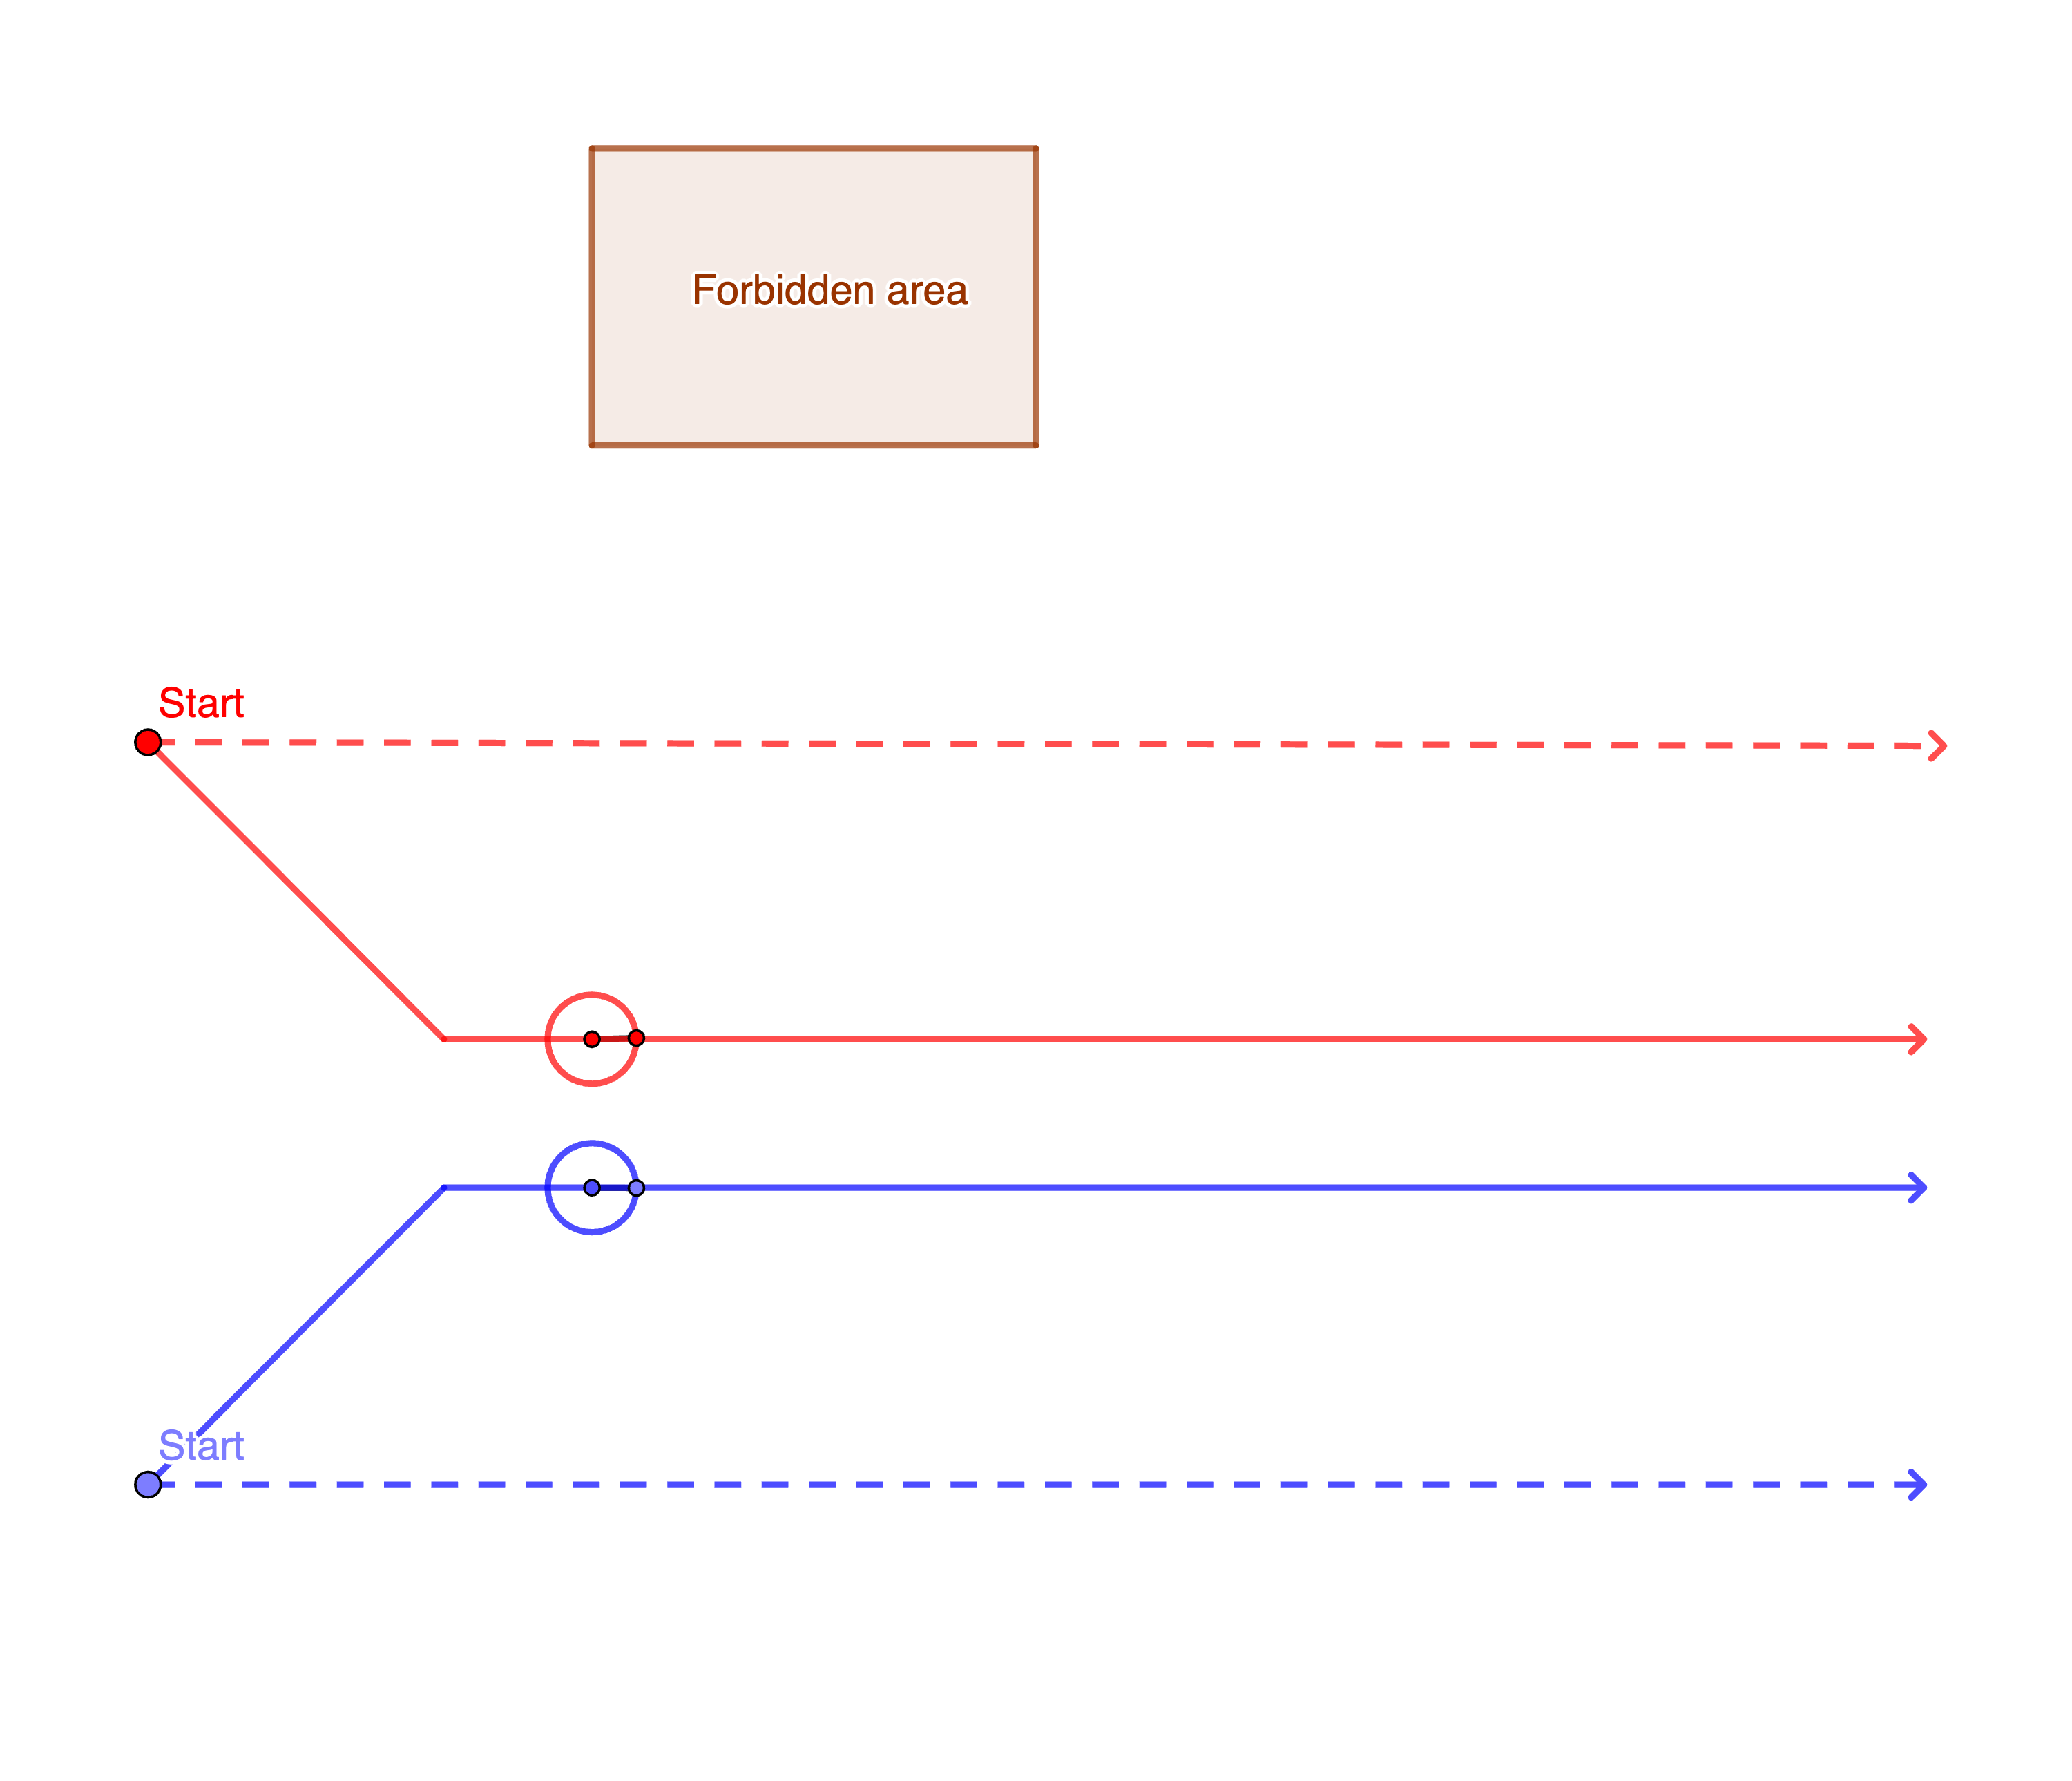
\includegraphics[width=0.45\linewidth]{co-observ}}
    \subfloat[Cross-trajectory co-observation \label{fig:example-cross-traj}]{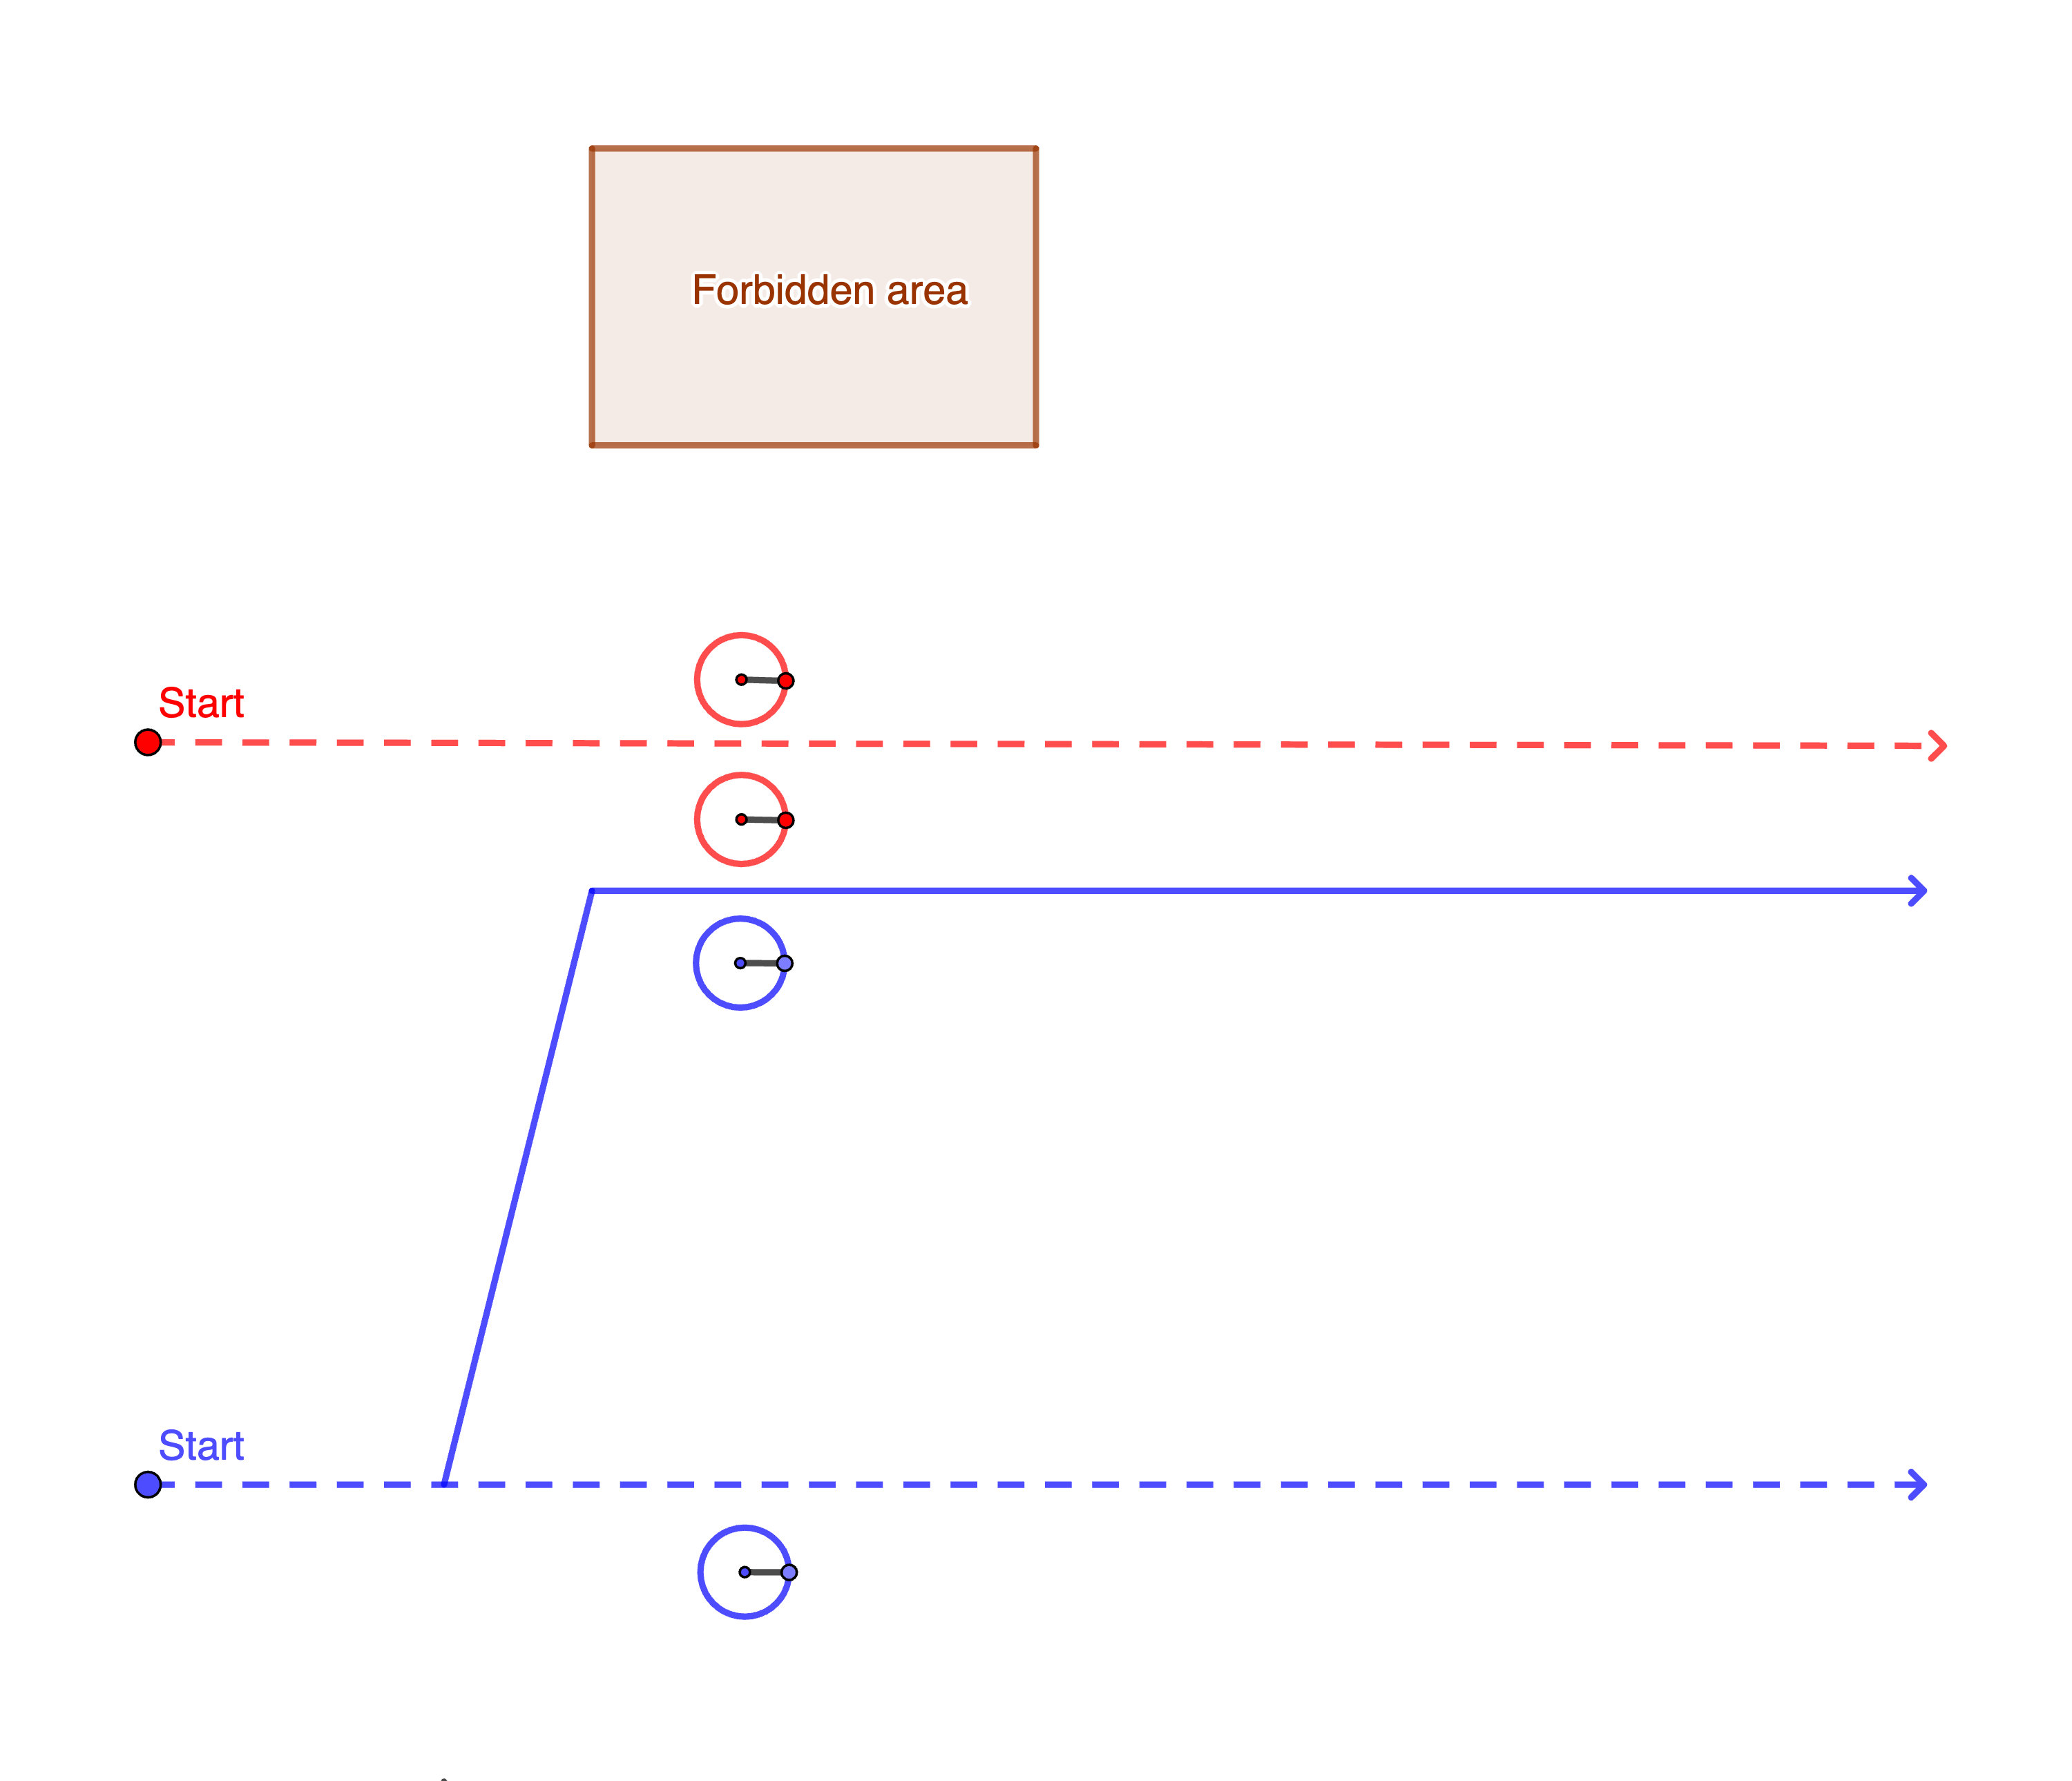
\includegraphics[width=0.45\linewidth]{cross-traj}}
    
    \caption{\ref{fig:example-co-observation} Limited by the co-observation requirement, both red and blue robot follow the co-observation secured routes (solid lines) and abandon the optimal ones (dashed line). \ref{fig:example-cross-traj} Through cross-trajectory co-observations, the blue team sends one robot to follow the red team (solid blue line) and performs co-observation while having the rest of the robots following the optimal trajectory.}\label{fig:cross-traj-comparison-set}
\end{figure}

\paragraph{Paper contributions} In this paper, we formulate a way to enforce an empty intersection between forbidden region and reachability regions, such that if an attacker takes control of the robots, they cannot perform an undetected attack by entering forbidden regions and meeting co-observation schedules at the same time. The constraints are formulated using an ellipsoidal bound of the reachability region. 

We propose to incorporate redundancy in the form of \emph{sub-team}s of multiple robots in place of individual robots along each route. This allows robots to deviate from their assigned sub-team, and join others to perform cross-trajectory co-observations, thereby securing multiple trajectories. We propose a formulation of the multi-flow problem on unsecured MRS trajectories to plan the cross-trajectory co-observations that can preserve the security against plan-deviation attacks.

\section{Preliminaries}
In this section, we review various mathematical concepts that will provide the foundations and context for our novel constraint.
\subsection{Ellipsoidal reachability constraints}\label{Chapter:ProblemFormulation}
  The reachability region is defined as the set of locations $x(t)$ that a robot can reach between two given fixed positions:

  \begin{definition}
    The \emph{reachability region} for two waypoints $x(t_1)=x_1$, $x(t_2)=x_2$ is defined as the sets of points $x'$ in the workspace such that there exist a trajectory $x(t)$ where $x(t')=x'$, $t_1\leq t' \leq t_2$ and $x(t)$ satisfies the velocity constraint $d(x(t),x(t+1))\leq v_{max}$.
  \end{definition}
  This region can be analytically bound via an ellipsoid:
  \begin{definition}\label{Def_Reachability}
    The \emph{reachability ellipsoid} is the region  $\mathcal{E}(x_1,x_2)=\{\tilde{x}\in\mathbb{R}^n: d(x_1,\tilde{x})+d(\tilde{x}+x_2)<2a\}$, where $a=\frac{v_{max}}{2}(t_2-t_1)$.
  \end{definition}
  % The reachability ellipsoid for a robot during time $[t_1,t_2]$ is the locations it could visit if only the planning at time $t_1$ and $t_2$ is obeyed.
  The region $\cE(x_1,x_2)$ is an ellipsoid with foci at $x_1,x_2$, center $o_{\cE} = \frac{1}{2}(x_1+x_2)$, and the major radius equal to $a$. Let $c_\cE=\frac{1}{2}\norm{x_1-x_2}=\norm{o_\cE-x_1}$ be the distance from the center to a foci.

  The reachability ellipsoid is an over-approximation of the exact reachability region; the difference between the two is due to the discretization of the trajectory, and the fact that $\cE$ does not consider the presence of obstacles.

\subsection{Rapidly-exploring Random Trees}
We use RRT* as a component of the solution \cite{karaman2010incremental}, which is an optimized variant of the rapidly-exploring Random Trees (RRT). As a optimal path planning algorithm, RRT* returns the shortest paths between an initial location and multiple potential goals. We assume that the generated paths can be travelled in both directions (this is used later in our analysis). The basic RRT* algorithm is shown in Algorithm \ref{alg:rrt}. For a given tree $G=(V,E)$, key functions called by the algorithm are
\begin{description}
\item[$\texttt{Sample}(i)$] This function returns independent identically distributed samples from the free configuration space.
\item[$\texttt{Nearest}(x)$] This function returns the vertex $v\in V$ that is closest in Euclidean distance to the input point $x$.
\item[$\texttt{Steer}(x,y)$] This function returns a point $z$ that minimize $\norm{z-y}$ subject to $\norm{z-x}\leq \eta$ for a prespecified $\eta>0$.
\item[$\texttt{ObstacleFree}(x,y)$] This function returns whether the line segment between $x$ and $y$ is free of collision.
\item[$\texttt{Cost}(v)$] This function assigns a non-negative cost (total travel distance in our application) to the unique path from the initial position to $v$ . 
\item[$\texttt{Parent}(v)$] This is a function that maps the vertex $v$ to $v'\in V$ such that $(v',v)\in E$
\end{description}

\begin{figure}[htbp]
\begin{center}
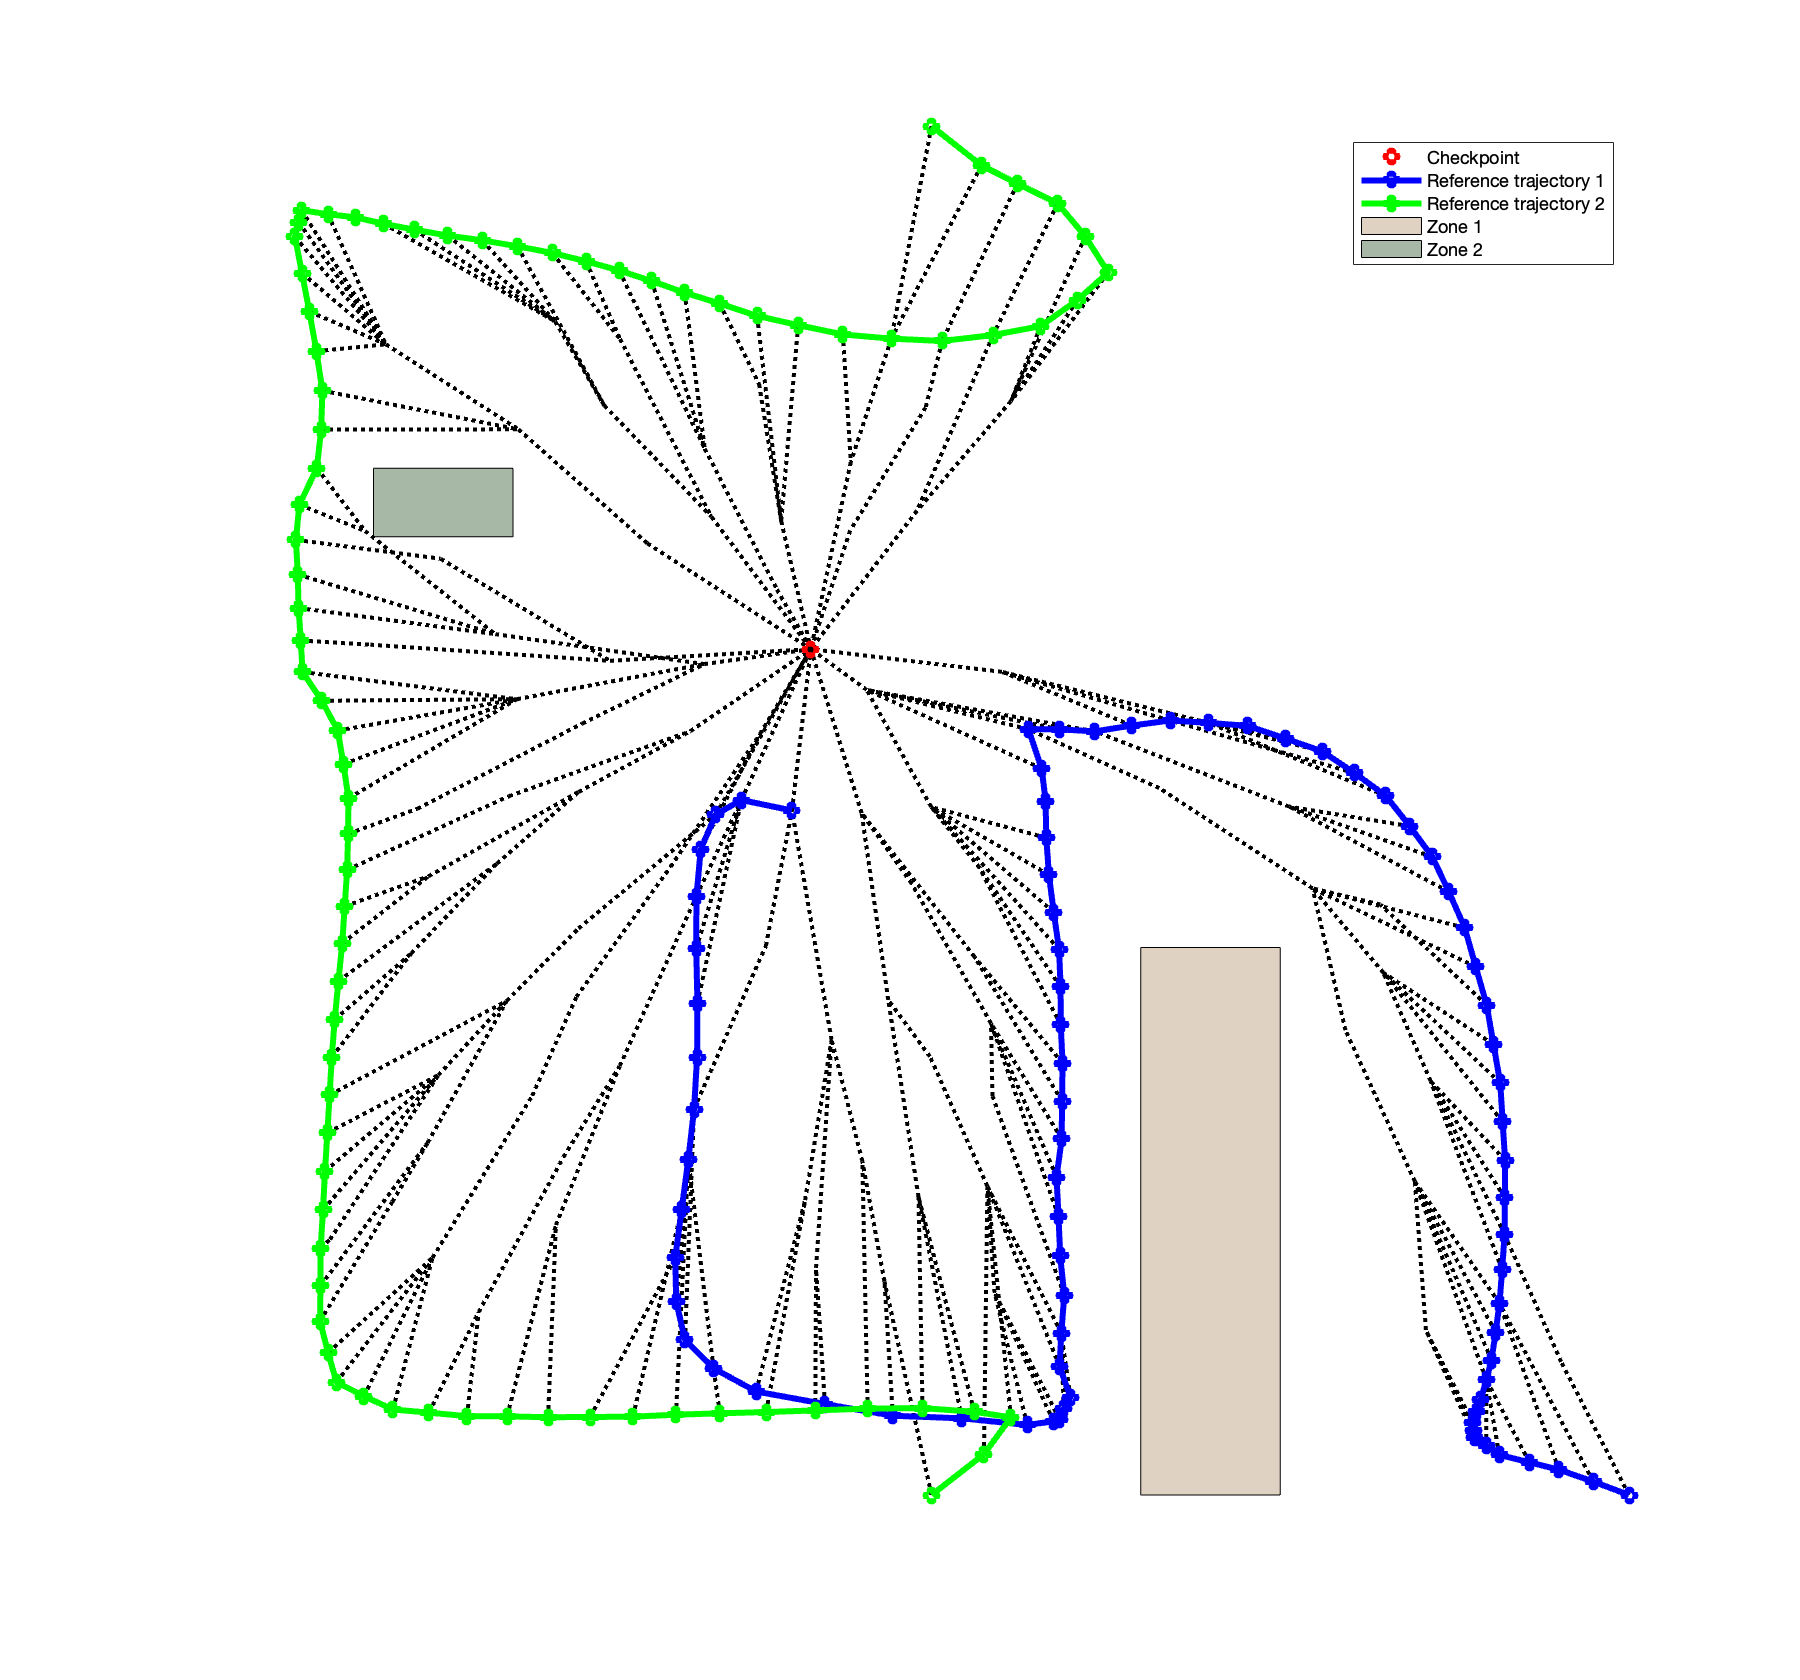
\includegraphics[width=0.8\linewidth]{RRT_example_new}
\caption{RRT* used to find trajectory from a point to different trajectories}
\label{fig:RRT*}
\end{center}
\end{figure}

	\begin{algorithm} 
		\caption{RRT*($x_{init}, \{x_{goal}\}$)} \label{alg:rrt}
		\begin{algorithmic}[1]
			\State $V_{goal}\gets\{x_{goal}\}$
			\State $V\gets x_{init} \union V_{goal} $, $E\gets 0$
			\State $i\leftarrow 0$
			\While{$i<N$}
			\State $G\leftarrow (V,E)$
			\State $x_{rand}\leftarrow \texttt{Sample}(i)$; $i=i+1$;
			\State $x_{nearest}\leftarrow \texttt{Nearest}(G=(V,E),x_{rand})$;
			\State $x_{new}\leftarrow\texttt{Steer}(x_{nearest},x_{rand})$;
			\If{$\texttt{ObstacleFree}(x_{nearest},x_{new})$}
			\State $V\leftarrow V\cup \{x_{new}\}$;
			\State $x_{min}\leftarrow x_{nearest}$;
			\ForAll{ $x_{near}\in X_{near}$}
				\If{$\texttt{ObstacleFree}(x_{near},x_{new})$}
					\State $c'\leftarrow \texttt{Cost}(x_{near})+c(\texttt{Line}(x_{near}, x_{new}))$;
					\If{$c'<\texttt{Cost}(x_{new})$}
						\State $x_{min}\leftarrow x_{near}$;
					\EndIf			
				\EndIf
			\EndFor
			
			\ForAll{$ x_{near}\in X_{near}\backslash {x_{min}} $}
				\If{$\texttt{ObstacleFree}(x_{new},x_{near})$ and $\texttt{Cost}(x_{near})>\texttt{Cost}(x_{new}+c(\texttt{Line}({x_{new},x_{near}})))$}
					\State $x_{parent}\leftarrow \texttt{Parent}(x_{near})$;
					\State $E' \leftarrow E' \backslash \{ (x_{parent}, x_{near})\}$;
					\State $E' \leftarrow E' \union  \{ (x_{new}, x_{near})\} $
				\EndIf
			\EndFor
			\EndIf
			\EndWhile
			\State \Return $V_{goal}$;
		\end{algorithmic}
	\end{algorithm}

\section{Problem overview}

Assume we have a total of $N$ robots in the system. We define a partition $\cI=\union_p \cI_p$ of the robots such that robots in \emph{sub-team} $\cI_p$ have the same nominal trajectory. We use the planner introduced in Chapter \ref{chapter:Multi-agent-ADMM} to generate multi-robot trajectories with $N_{p}<N$ routes $\{q_p\}_{p=1}^{N_p}$ without reachability and co-observation constraints, where the state $q_p(t), p \in\{0,\ldots,N_{p}\}$ represents the reference position of the $i$-th sub-team at time $t\in\{0, \dots, t_{e}\}$. Within each sub-team, at least one robot is required to follow the reference trajectory to fulfill the required tasks. Meanwhile, the additional robots can switch from one reference trajectory to another in order to perform co-observation with different sub-teams. We refer to the new type of co-observations as \emph{cross-trajectory co-observation}s. The goal is to find the cross trajectory co-observation plan to secure an unsecured MRS trajectory as with a minimal number of additional robots.

To solve this problem, we model the planned trajectory $\{q_p\}_{p=1}^{N_p}$ as a directed \emph{checkpoint graph} $G_{q}=(V_{q}, E_{q})$. Vertices $V_{q}$ are a key locations in $\{q_p\}$ that are used to perform co-observations. Part of these vertices are \emph{checkpoints} which are selected to guarantee that, if robots deviate and reach forbidden regions, they will miss the scheduled co-observations. Other vertices are selected to connect checkpoints on different trajectories. The set $E_{q} = E_{t} \union E_{c}$ consists of directed edges of two types, trajectory edges $E_{t}$ and cross-trajectory edges $E_{c}$, representing paths which robots can take. The trajectory edges $E_{t}$ represent the reference trajectories, where each edge connects two waypoints on the trajectory of the same sub-team. The cross-trajectory edges $E_{c}$ connect vertices on different reference trajectories, with at least one of the vertices being a checkpoint. These edges represent the potential paths that robots can take to travel and perform co-observations between trajectories of different sub-teams. Similar to the work done by \cite{yu2013multi}, we show that additional robots in the sub-team can be formulated as flows in the checkpoint graph, transforming the co-observation planning problem into a network multi-flow problem that can be solved using general linear programming techniques as specialized solver. 

In this chapter, we present a solution to the cross-trajectory co-observation planning problem. This approach consists of two components: constructing the checkpoint graph based on unsecured multi-robot trajectories, which includes the location of security checkpoints and cross-trajectory paths, and the formulation of the network flow problem to solve for the co-observation plan.
\section{Checkpoint graph construction}

In this section, we describe in detail how we define and search for security checkpoints and use the checkpoints to find cross-trajectory edges and construct a directed security graph $G_{q}=(V_{q},E_{q})$.

\subsection{Checkpoints}\label{sec:security-checkpoint}
Let $q\in\real{nmT}$ be the MRS trajectory found in Chapter \ref{chapter:Multi-agent-ADMM} for $m$ sub-teams with time horizon $T=t_{e}$, with $q_{p}(t)$ be the reference trajectory waypoint for sub-team $p$ at time $t$. A checkpoint $v_i=(q_{i},t_{i})$ is a pair composed of a location $q_{i}=q_{p}(t_{i})$ and a time $t_{i}$ representing a co-observation between a sub-team $\cI_p$'s member and robots either from the same sub-team or different ones. For convenience, let $\cI_{v_{i}}$ represent the corresponding sub-team $v_{i}$ belongs to. 

Similar to the requirements of co-observations introduced in Chapter \ref{chapter:Reachability_Constraints}, checkpoints $V_{p}=\{ v_{p_{1}}, \dots ,v_{p_{e}}\} \subset V_{q}$ for a reference trajectory $\{q_{p}(t)\}$ of sub-team $p$ need to guarantee that the reachability region between consecutive checkpoints $\mathcal{E}(q_{p_{i}}, q_{p_{i+1}}, t_{p_{i}},t_{p_{i+1}})$ does not intersect with any of the forbidden areas. For convenience, we denote the union of all forbidden areas as $F$; then the requirement can be written as $\mathcal{E}(q_{p_{i}}, q_{p_{i+1}}, t_{p_{i}},t_{p_{i+1}}) \intersect F = \emptyset$, for every $i$. 

We provide a heuristic approach to locate the checkpoints on given trajectories; an optimal solution would likely be NP-hard, while the approach below works well enough for our purpose. We begin by adding the start and end locations $q_{p}(t_{0})$, $q_{p}(t_{e})$ to $V_{q}$, where $t_{0}=0$, and $t_{e}$ is the time horizon. Then, we search for the waypoint $q_{p}(t_{1})$ with the largest $t_{1} \in \{t_{0}, \dots ,t_{2}\}$ such that the reachability ellipsoid between $q_{p}(t_{0})$ and $q_{p}(t_{1})$ has no overlap with any of the forbidden areas, i.e. $\mathcal{E}(q_{p}(t_{0}),q_{p}(t_{1}), t_{0},t_{1})\intersect F = \emptyset$. Simultaneously, we search backward to find $q_{p}(t_{3})$ with the smallest $t_{3}\in \{t_{1}, \dots ,t_{2}\} $ that meets the reachability requirement $\mathcal{E}(q_{p}(t_{2}),q_{p}(t_{3}),t_{2},t_{3}) \intersect F = \emptyset$. $q_{p}(t_{1})$ and $q_{p}(t_{3})$ are then added to $V_{q}$. Afterwards, we set $t_{0}=t_{1}$, $t_{2}=t_{3}$ and repeat the same process. The search is stopped when $t_{0}>t_{2}$, or when $\mathcal{E}(q_{p}(t_{0}),q_{p}(t_{2}),t_{0},t_{2}) \intersect F = \emptyset$. A toy example is shown in Figure \ref{fig:checkpoint-generate}. 

\begin{figure}
	\centering
    \subfloat[]{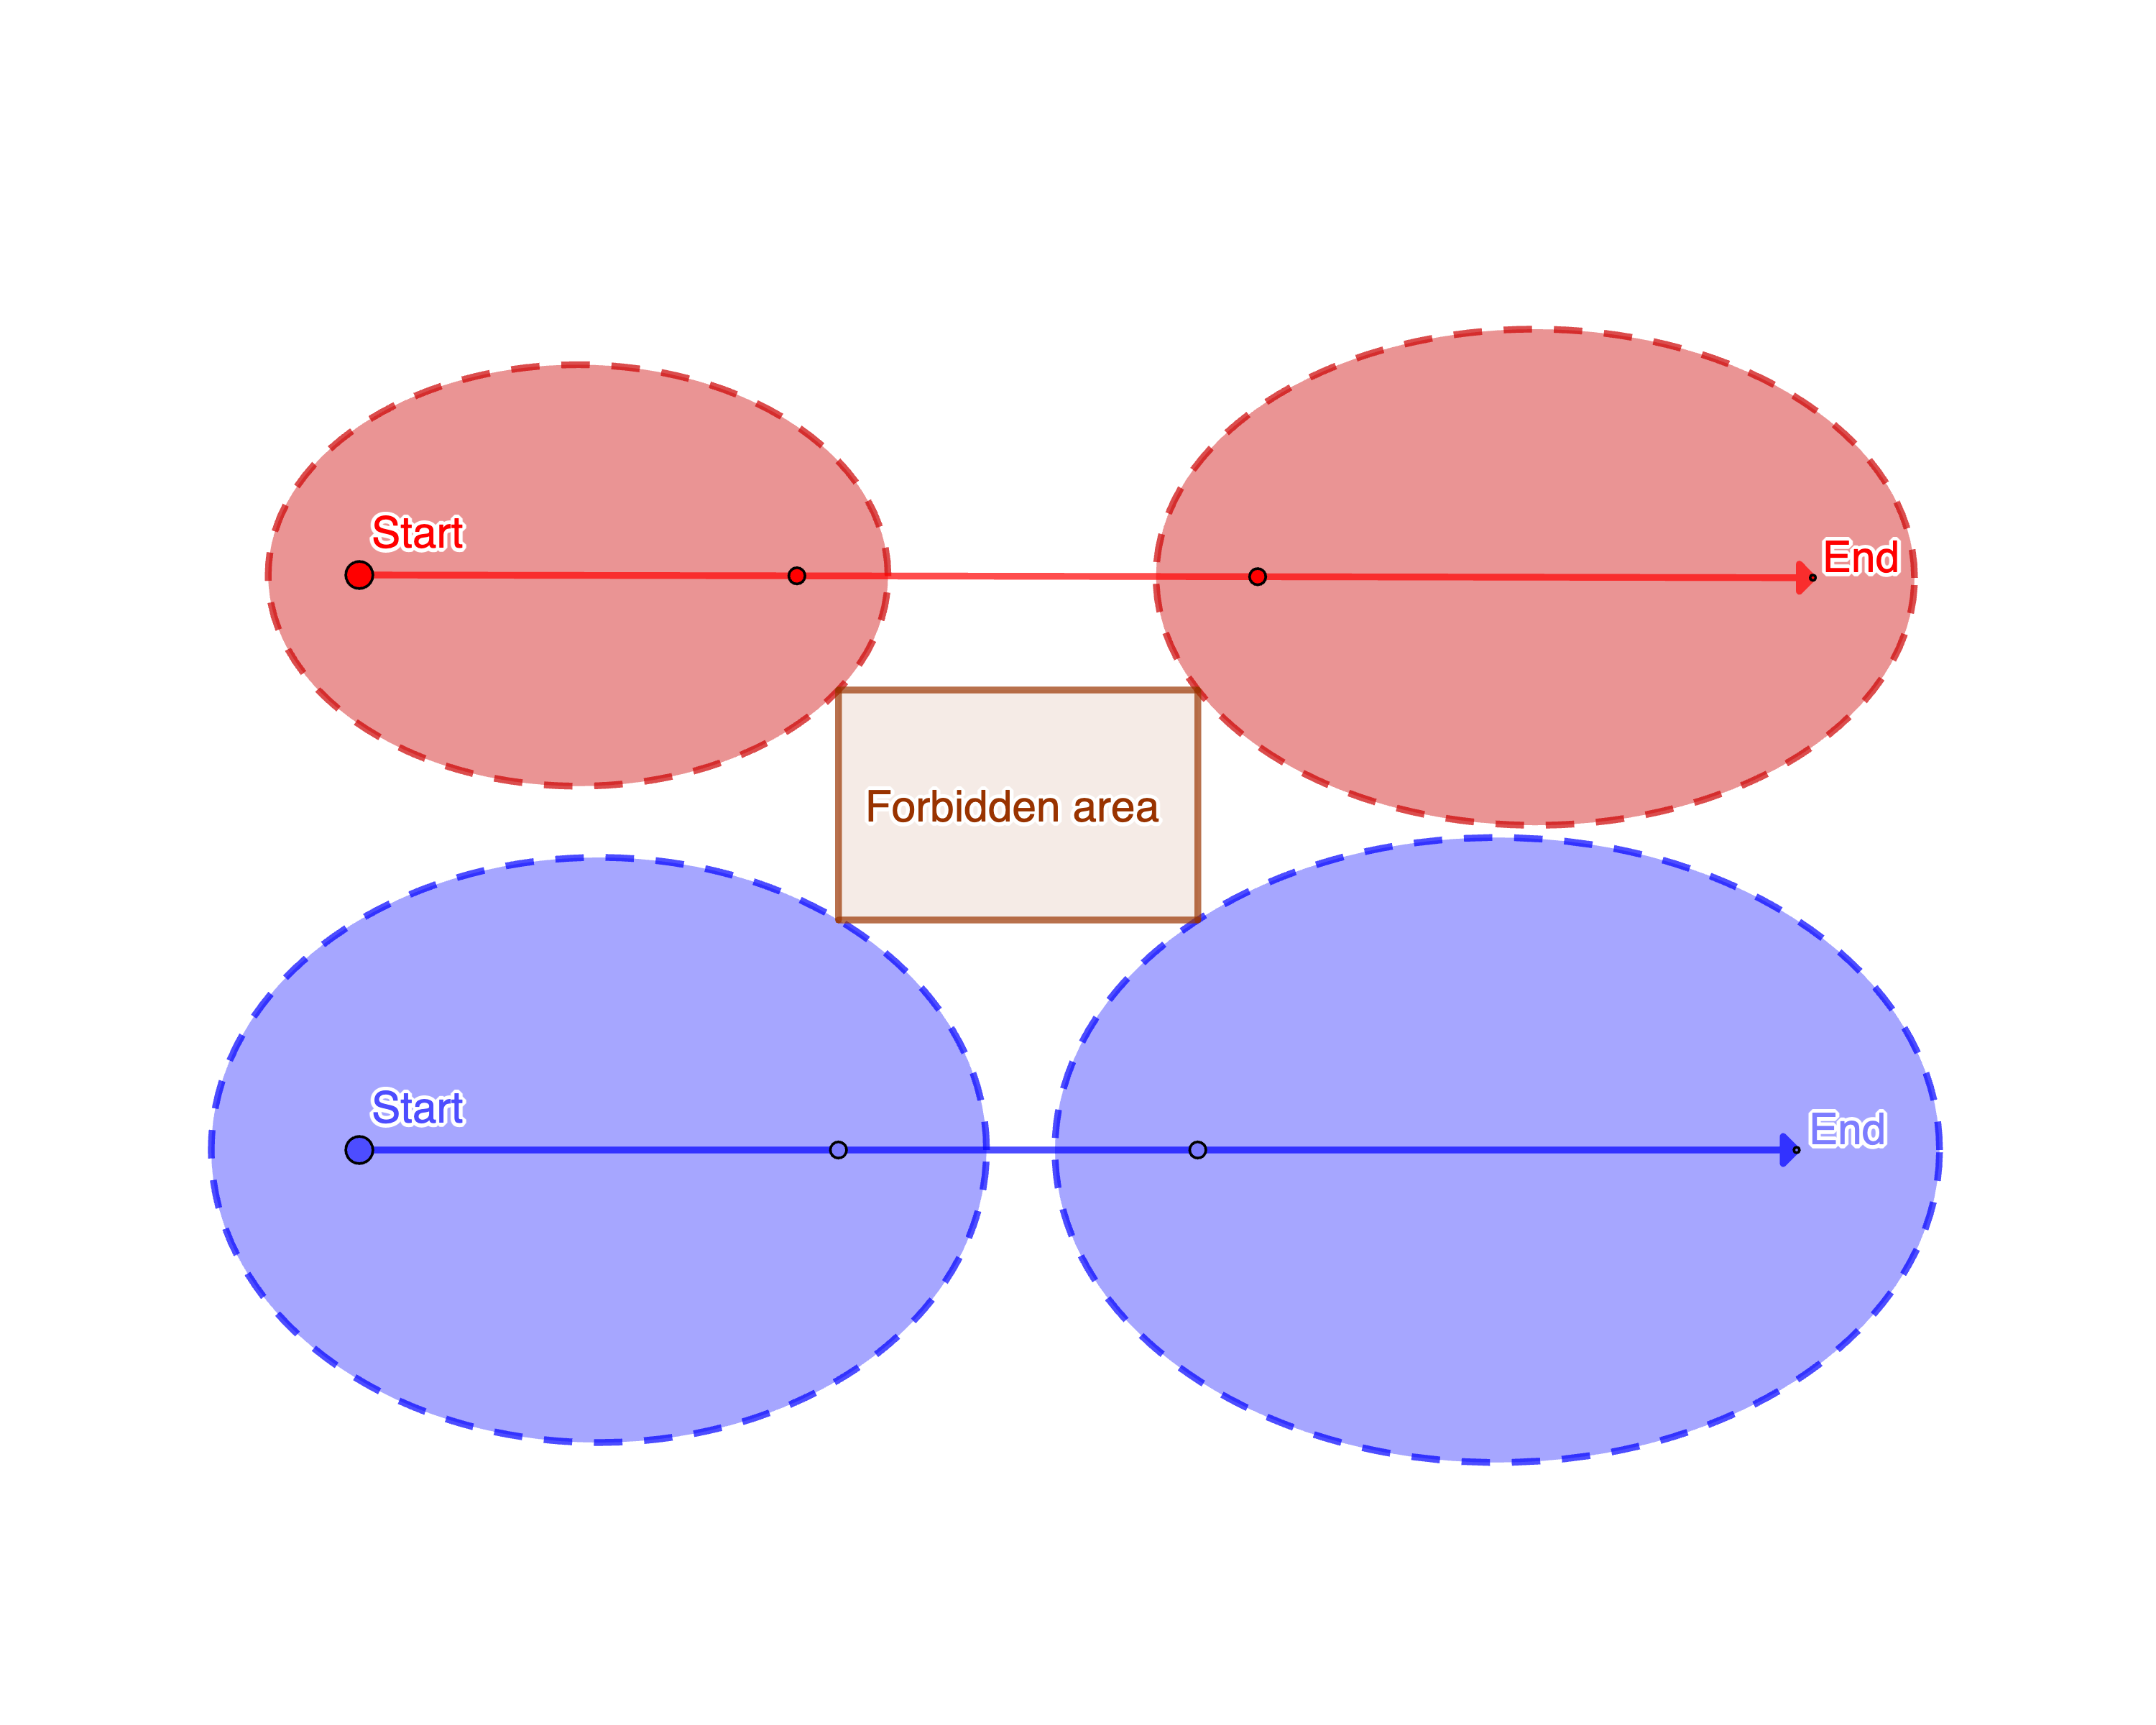
\includegraphics[width=0.45\linewidth]{SC_gen_1}}
    \subfloat[]{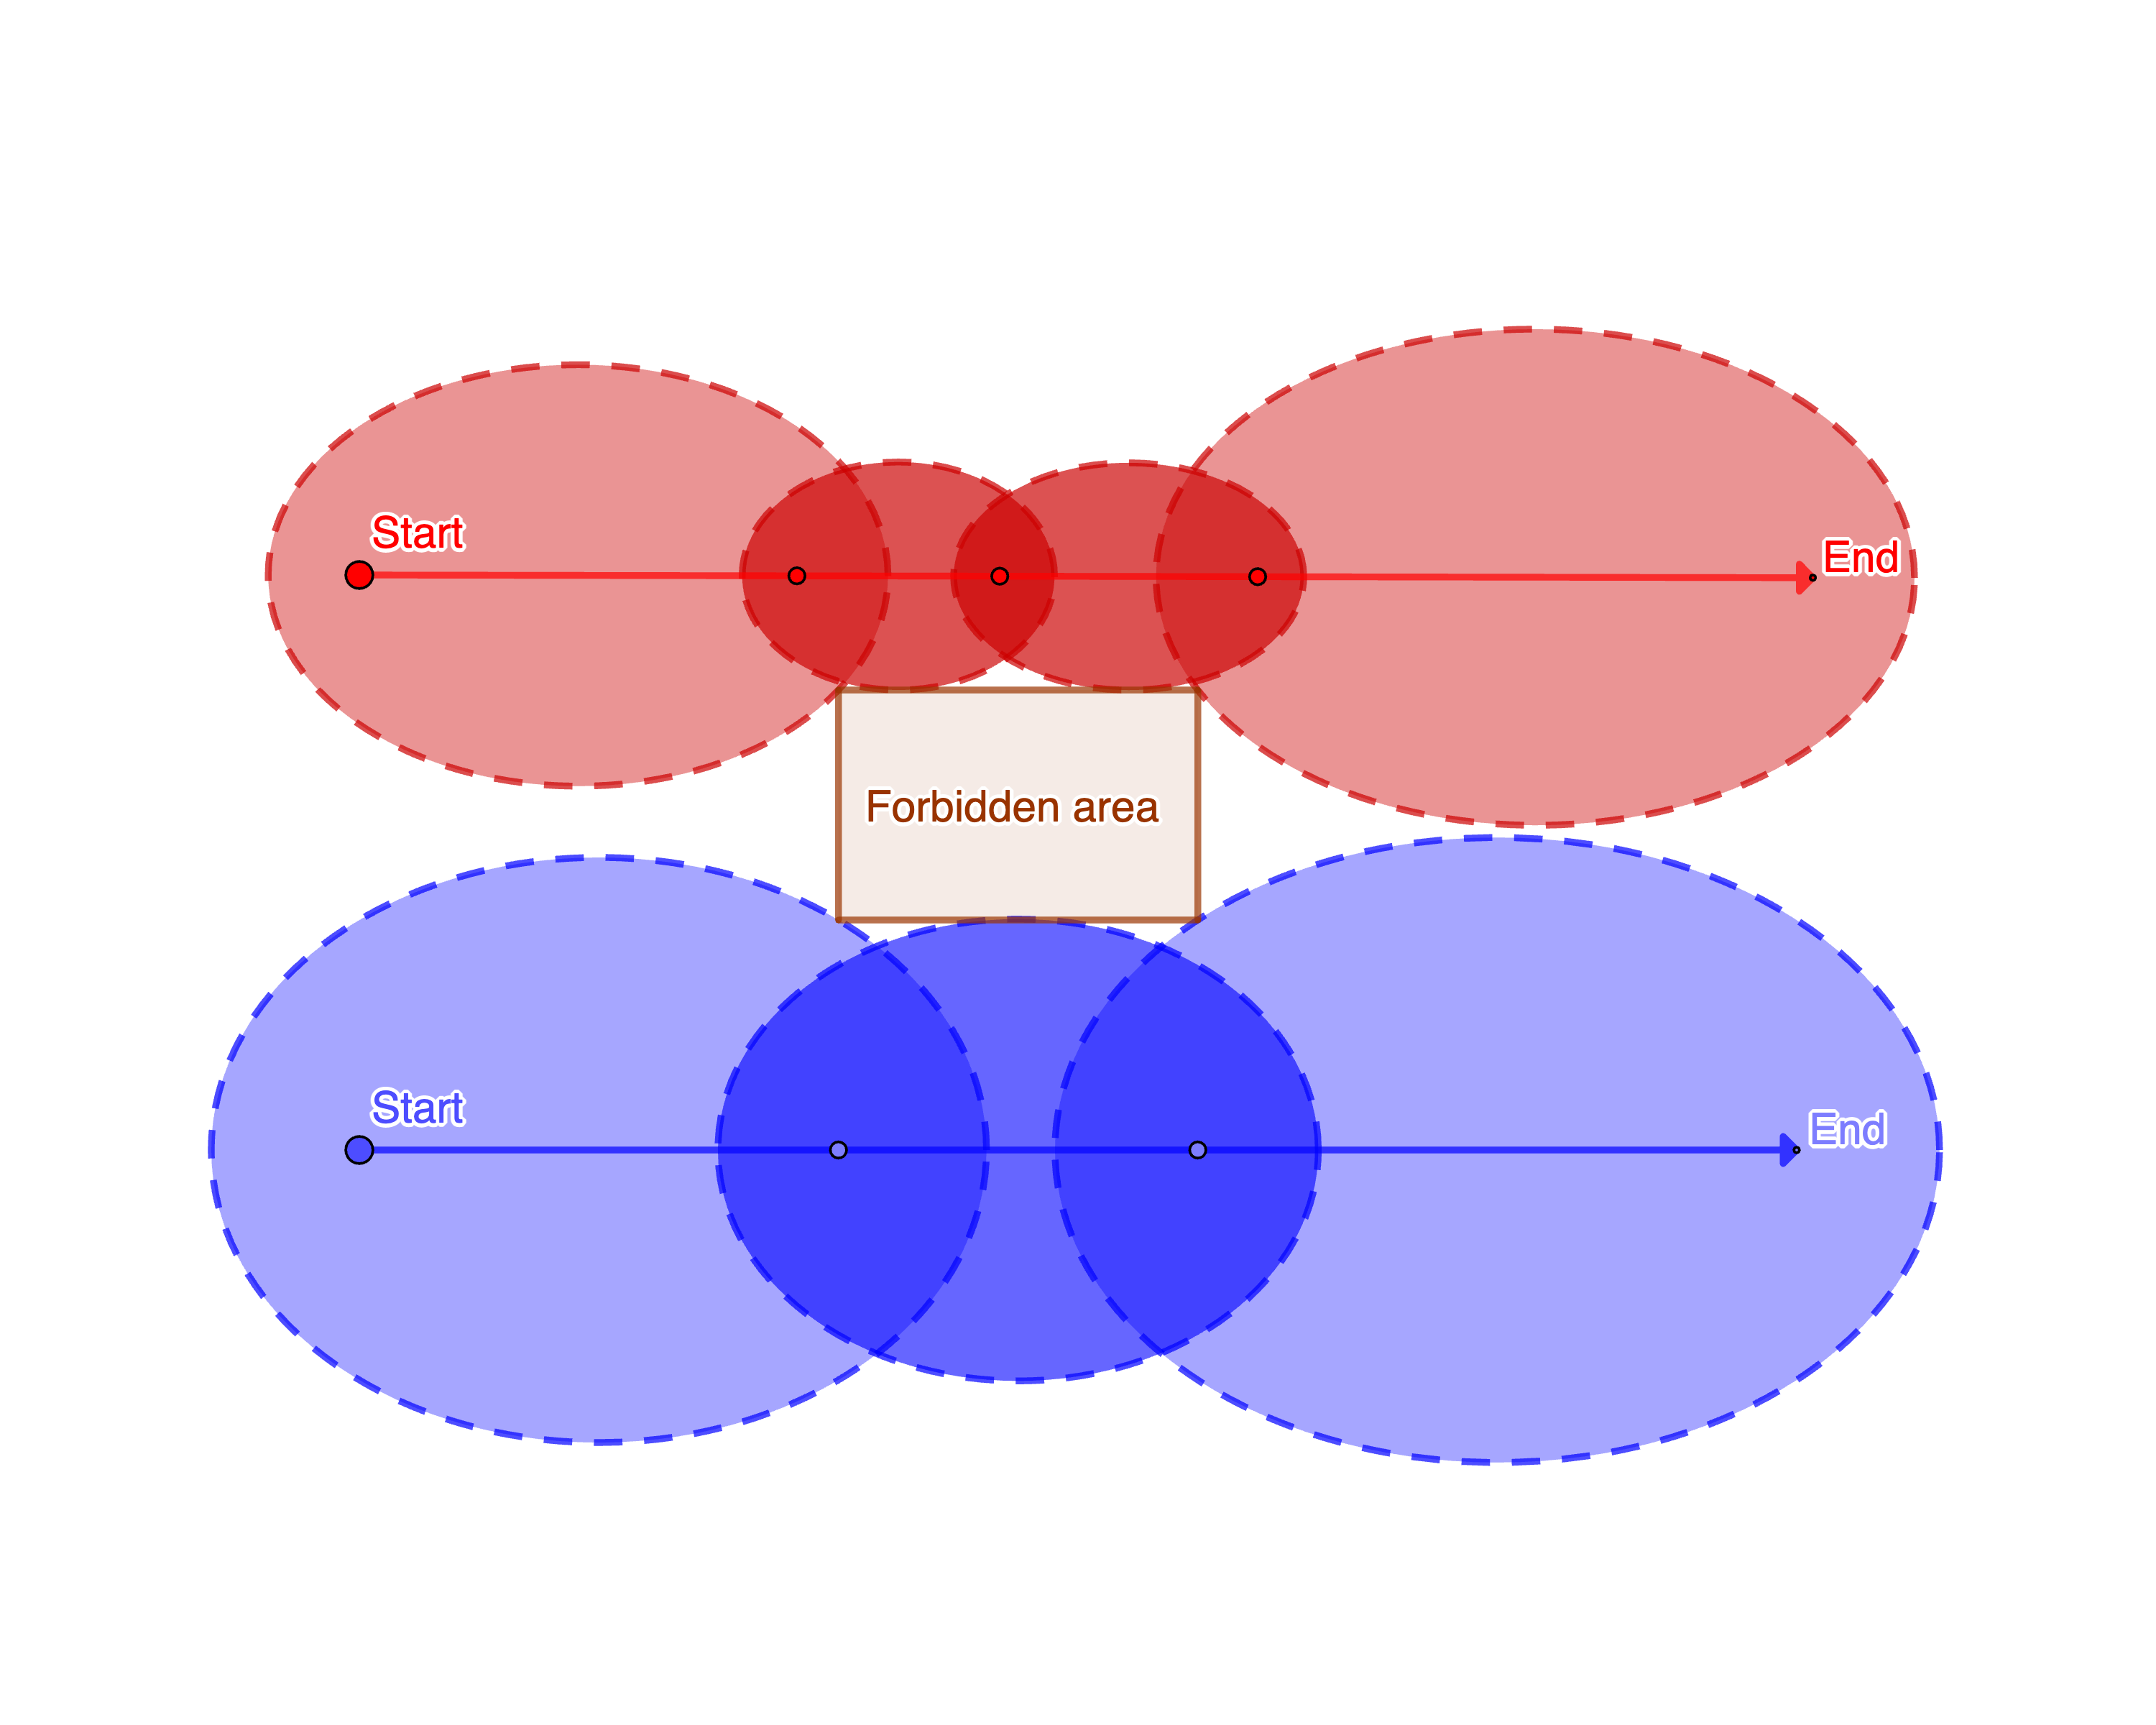
\includegraphics[width=0.45\linewidth]{SC_gen_2}}
    \caption{Checkpoint generation example}\label{fig:checkpoint-generate}
\end{figure}

\subsection{Cross-trajectory edges}\label{sec:cross-traj-edges}
After locating checkpoints $\union_p V_p$ for all sub-teams, we can search for cross-trajectory edges to connected all checkpoints to trajectories. Cross-trajectory edges represents feasible paths between two references trajectories that allow robots to reach a different reference trajectories and perform co-observations with the corresponding sub-teams. Thus, at least one end of the edges must be a security checkpoint $v_{p} \in \union_p V_p$. Additionally, assuming that only one robot is sent at a time between trajectories, the cross-trajectory edges must satisfy the reachability constraints from Chapter~\ref{chapter:Reachability_Constraints} to ensure that no deviation to forbidden areas can be performed while switching trajectories.  

\begin{figure}[htbp]
\begin{center}
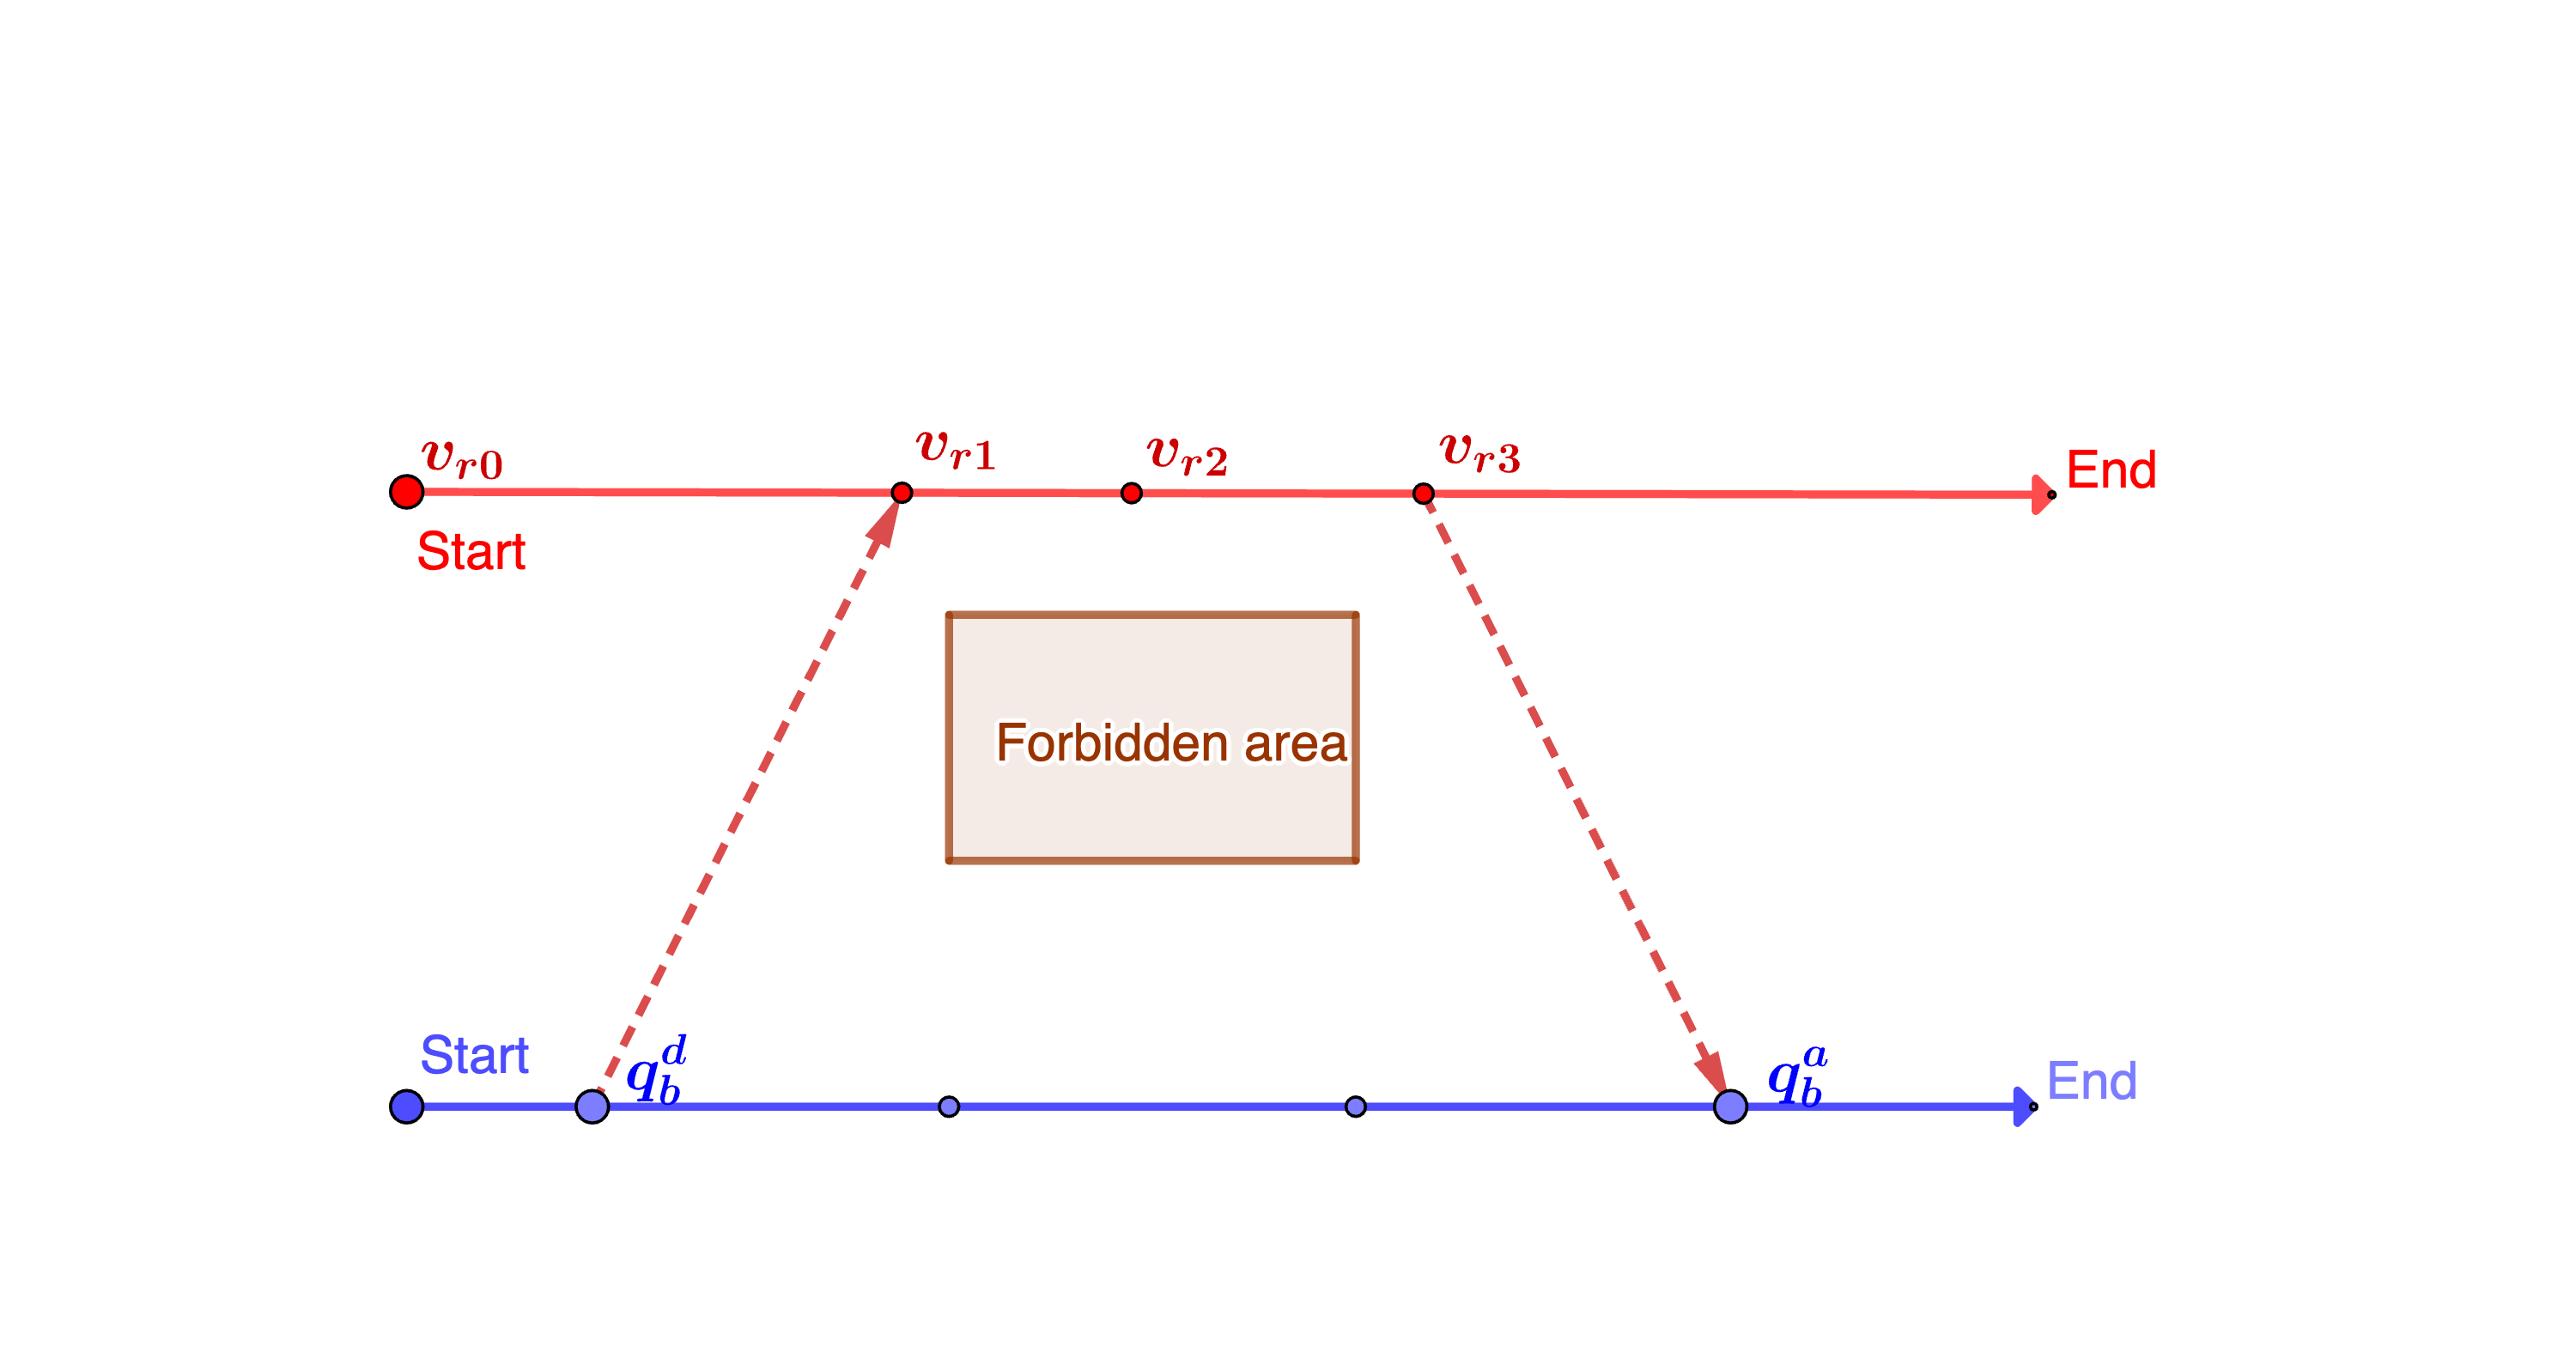
\includegraphics[width=0.6\linewidth]{two_edges}
\caption{For checkpoints of the red trajectory, latest departure node $q^{d}_{b}$ found for $v_{r1}$ and earliest arrival node $q^{a}_{b}$ found for $v_{r3}$.}
\label{fig:two-edges}
\end{center}
\end{figure}

To find cross-trajectory edges, we base our approach on RRT*. First, we search for feasible paths between each security checkpoint in each reference trajectory and all other trajectories, as shown in Figure \ref{fig:RRT*}. Since paths returned by RRT* are optimal and bidirectional, we can analyze the travel time and reachability for each candidate cross-trajectories, and  add these edges to the checkpoint graph if they are feasible.

More vigorously, After a fixed iterations of RRT*, we find all possible and close to optimal paths between one security checkpoint $v_{p}=(q_{p},t_{p}) \in V_{p}$ for sub-team $\cI_p$, and $V_{r} = \{ (q_{{r}_{i}}, t_{{r}_{i}}) \}$ where  $q_{{r}_{i}} = q_{r}(t_{{r}_{i}})$ are the entire waypoints on a reference trajectories for a different sub-team $\cI_{r}$ for a fixed number of RRT* iterations. We can calculate the minimal travel time $t=\texttt{Cost}(q)/v_{max}$ for a robot to traverse each path. We call all nodes $v_{{r}_{i}} \in V_{r}$ \emph{arrival node}s if there exist a path between $v_{{r}_{i}}$ and $v_{p}$ with $t_{p}+t<t_{{r}_{i}}$, and the reachability ellipsoid $\mathcal{E}(q_{r}(t_{{r}_{i}}),q_{p},t_{{r}_{i}},t_{p}) \intersect F = \emptyset$. Similarly, \emph{departure node}s are defined for $v_{{r}_{i}}$ with $t_{p}>t_{{r}_{i}}+t$ and $\mathcal{E}(q_{p}, q_{r}(t_{{r}_{i}}),t_{p}, t_{{r}_{i}}) \intersect F = \emptyset$. Given a point $v_{p} \in V_{p}$, we define the \emph{latest departure node} $q_{r}(t^{d}_r)$, and the \emph{earliest arrival node} $q_{r}(t^{a}_r)$ as follows:

\begin{description}
\item[Latest departure node $q_{r}(t^{d}_r)$]: is the waypoint with the latest time $t^{d}_r$ such that a robot from sub-team $\cI_r$  can meet with robots in sub-team $\cI_p$ at $v_{p}$.
\item[Earliest arrival node $q_{r}(t^{a}_r)$]: is waypoint with the earliest time $t^{a}_r$ such that a robot from sub-team $\cI_p$ deviating from $v_{p}$ can meet with sub-team $\cI_r$.
\end{description}

For $v_{p} \in V_{p}$, latest departure node $v_{d}=(q_{r}(t^{d}_r),t^{d}_r)$ and earliest arrival node $v_{a}= (q_{r}(t^{a}_r),t^{a}_r)$, if feasible, are added to $V_{q}$. Cross-trajectory edges $(v_{p} \to v_{a})$ and $(v_{d} \to v_{p})$ are added to $E_{q}$. Examples are shown in Figure \ref{fig:two-edges}. Full algorithm is shown in Algorithm \ref{alg:cross-trajectory-edges}.

\begin{algorithm}
\caption{Cross-trajectory edges generation}\label{alg:cross-trajectory-edges}
\begin{algorithmic}
\Procedure{CrossTrajectoryEdges}{$V$}
\State $V_{q} \gets V$; $E_{q}\gets 0$;
\ForAll {$v\in V$}
	\ForAll{$\vq_{r}$ that $\cI_{r} \neq \cI_{v}$}
		\State $V_{q},E_{q} \gets \textsc{AddEdges} (q_{v}, \vq_{r}, V_{q}, E_{q}) $;
	\EndFor
\EndFor
\State \Return $V_{q}, E_{q}$
\EndProcedure
\Procedure{AddEdges}{$q_{v}, \vq_{r}, V_{q},E_{q}$}
\State $t^{d}_r \gets -\infty $; $t^{a}_r \gets \infty$;
\State $\cV_{goal}=RRT^*(q_{v}, \vq_{r})$;
    \ForAll{$ q \in \cV_{goal} $ that $\texttt{Parent}(q)\neq \emptyset $}
        \If{$\texttt{Cost}(q)/ v_{max} < t_{q}-t_{v}$ and $\cE(q, v_{p},t_{q}, t_{v_{p}})\union F = \emptyset$}
        		\If{$t_{q}<t^{a}_r$}
			\State $t^{a}_r \gets t_{q}$;
		\EndIf
        \ElsIf{$\texttt{Cost}(q)/ v_{max} < t_{v} - t_{q}$ and $\cE(q, v_{p},t_{q},t_{v_{p}})\union F = \emptyset$}
        		\If{$t_{q}>t^{d}_r$}
			\State $t^{d}_r \gets t_{q}$;
		\EndIf
        \EndIf
    \EndFor
    \If{$t^{d}_r \neq -\infty $ and $t^{a}_r \neq \infty$}
    \State $v_{a} \gets (q(t^{a}_r),t^{a}_r)$; $v_{d} \gets(q(t^{d}_r), t^{d}_r)$;
    \State $V_{q}\gets V_{q} \union v_{a}$; $V_{q}\gets V_{q} \union v_{d}$;
    \State $E_{q}\gets E_{q} \union (v_{p} \rightarrow v_{a})$; $E_{q}\gets E_{q} \union (v_{d} \rightarrow v_{p})$
    \EndIf
    \State \Return $V_{q},E_{q}$
    \EndProcedure
   \end{algorithmic}
\end{algorithm}

\subsection{In-trajectory edges}\label{sec:Graph-intro}

%With vertices $V_{q}$ and cross-trajectory edges $E_{q}$ found in Algorithm \ref{alg:cross-trajectory-edges}, we can construct a security graph $G_{q}$. 
All checkpoints $V_{q}$ found in Section~\ref{sec:security-checkpoint} and \ref{sec:cross-traj-edges}, can be divided by the corresponding sub-team and sorted in ascending order of time into $N_{p}$ subsets $V_{p}=\{v^{p}_{0}, v^{p}_{1}, \dots , v^{p}_{T}\}$ where $p\in \{1,\dots, N_{p}\}$. Consecutive edges in the same subset are added to $E_{q}$ as in-trajectory edges $(v^{p}_{i}\rightarrow v^{p}_{i+1} )$. Example are shown in Figure \ref{fig:security-graph-generate}.
\begin{figure}[htbp]
\begin{center}
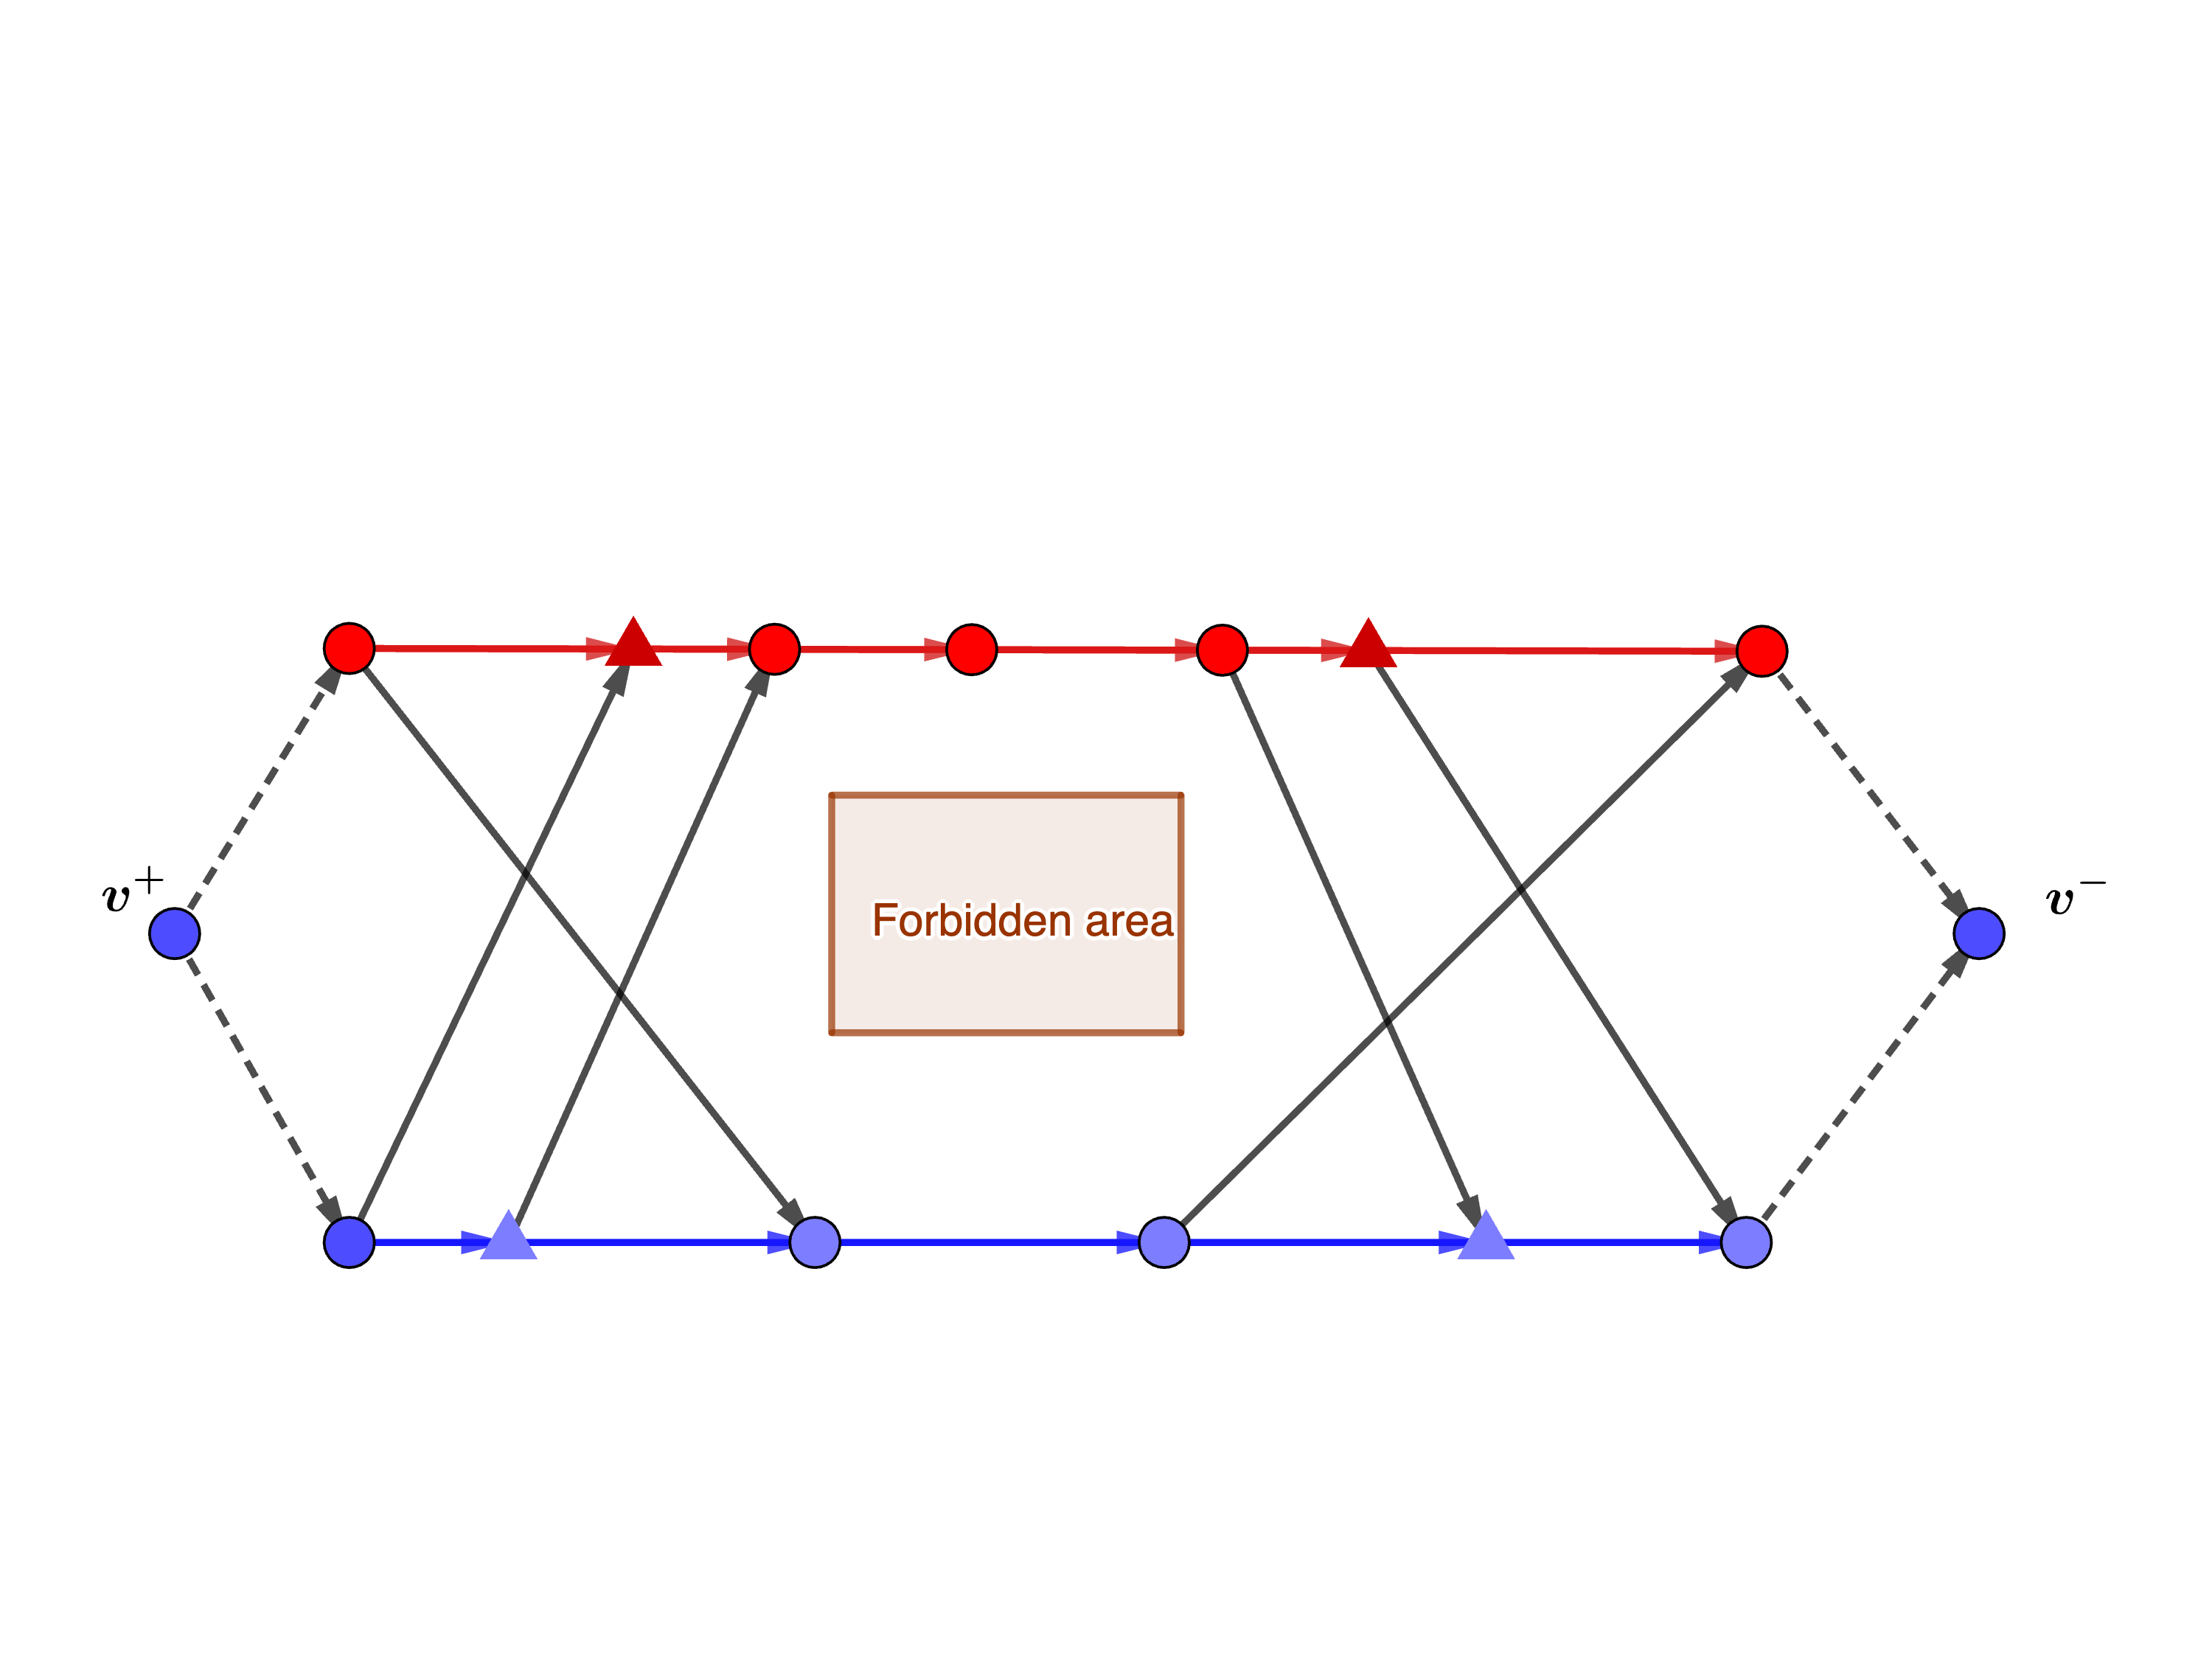
\includegraphics[width=0.6\linewidth]{security_graph}
\caption{Example of a two trajectory security graph. Round vertices are checkpoint generated through the heuristic search and triangle vertices are added with the cross-trajectory edges. Additional virtual source $v^{+}$ and sink $v^{-}$ is used later in planning problem.}
\label{fig:security-graph-generate}
\end{center}
\end{figure}

%For convenience, we use $|V_{q}|$ and $|E_{q}|$ to denote the cardinality of the sets $V_{q}$ and $E_{q}$ 

\section{Co-observation planning problem}
In this section, we describe in detail how to formulate the cross-trajectory planning problem as a network flow problem, and solve it using mixed-integer linear programs (MILP). We assume that there are always \emph{reference robot}s in each sub-team following the reference trajectory.  We want to plan the routes for additional \emph{cross-trajectory robots} to perform co-observation with the reference robots. 

To formulate the planning problem as a network multi flow problem, we augment the checkpoint graph $G_{q}$ to a flow graph $G=(V, E)$. The vertices of the new graph are defined as $V= V_{q} \union \{v^{+},v^{-}\}$,  a \emph{virtual source} $v^{+}$ and a \emph{virtual sink} node $v^{-}$ are added to $V$. The edges of the new graph are defined as $ E = E_{q} \union \{( v^{e}_{p},v_{-})\}_{p} \union \{(v_{+},v^{0}_{p})\}_{p}$, where directed edges are added to $E$ from $v^{+}$ to all the start vertices, and from all end vertices to $v^{-}$, with $v^0_p$ and $v^e_p$ representing the start and end vertices of sub-team $\cI_p$.

Assume that all the robots starting from the virtual source $v^{+}$ and end in the virtual sink $v^{-}$. Each robot may move from vertex $v_{i}$ to $v_{j}$ if $(v_{i},v_{j})\in E_{q}$. The path of a robot $k$ can be represented as a flow vector $\vf^{k} = \{ f^{k}_{ij} \}$, where $f^{k}_{ij} \in \{1,0\}$ is an indicator variable representing whether robot $k$'s path contains the edge $(v_{i},v_{j})$. As required by the security guarantee, reference robots must be seen by at least one surveillance robot at every checkpoint. Thus, the planning problem can then be formulated as a path cover problem on $G_{q}$, i.e., as finding a set of paths $F=[\vf_{1},\dots, \vf_{\cK}]$ for cross-trajectory robots such that every checkpoint in $V_{p}$ is included in at least one path in $F$. Additionally, to encourage the robots' exchange between different sub-teams, cross-trajectory co-observations are preferred compared to co-observation within the same team. This is achieved with the weights for edges $(v_{i},v_{j})\in E$ defined as:
\begin{equation}
	w_{i,j}=\begin{cases}
	-w_{t} & \cI_{v_{i}}=\cI_{v_{j}}, (v_{i},v_{j})\in E_{q}\\
	w_{c} & \cI_{v_{i}} \neq \cI_{v_{j}}, (v_{i},v_{j})\in E_{q}\\
	0 &  (v_{i},v_{j})\in E / E_{q} 
	\end{cases}
\end{equation}
where $w_{c} > w_{t}$. 

With the formulation above, the planning problem can be written as an optimization problem, where we want to balance between the co-observation performance and total number of flows (cross-trajectory robots) needed. For convenience, we use $(ij)$ to represent the edge $(v_{i},v_{j})$, and $(+i)$ to represent the edge $(v^{+},v_{i})$.

 \begin{subequations} \label{eq:flow-coverage-problem}
     \begin{align}
        \min &\quad \sum^{\cK}_{k} \sum_{(+i)\in E} f^{k}_{+i} - \rho \sum^{\cK}_k \sum_{(ij)\in E} w_{ij} f^k_{ij} &\label{eq:flow-cost}\\
        \subjectto & \sum_{\{h:(hi) \in E\}}f^k_{hi}=\sum_{\{j:(ij) \in E\}}f^k_{ij}, & \forall k,\forall v \in V_{q} / \{v^{+}, v^{-}\}  \label{eq:FlowBalanceConstraint}\\
        & \sum^{\cK}_k\sum_{\{i:(ij)\in E \}} f^k_{ij} \geq 1 & \forall v_{j} \in \{V^{s}_{p}\} \label{eq:FlowCoverage}\\
        & f^k_{ij} \in \{0,1\} &  \forall (ij)\in E\label{eq:SingleFLowCapacity}
     \end{align}
 \end{subequations}

The first term in \ref{eq:flow-cost} is total outgoing flow from the source $v^{+}$ while the second term is the total cost of all flows which represents the overall co-observation performance (defined as the total number of cross-trajectory edges taken by all flows beyond the regular trajectory edges). The constant $\rho$ is a penalty parameter manually elected to balance between two terms in the cost function. The constraint \eqref{eq:FlowBalanceConstraint} is the flow conservation constraint, which ensures that the amount of flow entering and leaving a given node $v$ is equal (except for $v^{+}$ and $v^{-}$). The constratin \eqref{eq:FlowCoverage} is the flow coverage constraints, which ensures that all security checkpoints $ \{V^{s}_{p}\}$ have been visited by at least one flow (robot). Since the security graph $G_{q}$ is acyclic, this problem is in complexity class $P$, and can be solved in polynominal time \cite{ntafos1979path}. 

\section{Co-observation performance}
Notice that problem \eqref{eq:flow-coverage-problem} is guaranteed to have a solution for $\cK=N_{p}$ where all $\cK$ robots follows the reference trajectory ($f^{k}_{ij}=1, \forall \cI_{v_{i}}=\cI_{v_{j}}=k$).  Additionally, for a fixed number of robots $\cK \geq N_{p}$, it is possible to have a subset of flows $F_{\cE} \in F$ that is empty, i.e. $f_{ij}=0, \forall (v_{i},v_{j})\in E$, $f\in F_{\cE}$, these flow will not increase the cost and will not have any impact on the solution.  
The trade-off between the number of surveillance robots used, and the overall security performance is a critical consideration in this case. Increasing the number of robots generally contributes to improved security by enabling more cross-trajectory co-observations. However, adding more robots can lead to diminishing returns, as the benefits gained from additional robots may be counterbalanced by increased complexity and coordination challenges. To capture this trade-off, the penalty parameter $\rho$ in the cost function \ref{eq:flow-cost} allows us to fine-tune the balance between the number of robots employed and the desired task performance. By optimizing this parameter, we can strike a suitable equilibrium between security enhancement and operational efficiency.

To find such tradeoff, we employ an iterative approach. We start with $\cK=1$ and gradually increase it until $F$ contains a empty flow. This indicates that the performance can no longer be improved by adding more robots. To ensure that the value of $\cK$ does not grow unbounded, penalty parameter $\rho$ need to ensure that the second term for a single flow in \eqref{eq:flow-cost} $ \rho \sum_{(ij)\in E} w_{ij} f^k_{ij}$ is always smaller than $1$.

\section{Result and simulation}
In this section, we test the proposed method starting from the results in Figure \ref{fig:trajectories-more-constraint}, where three trajectories are provided for the map exploration task with no security related constraints (co-observation schedule and reachability). We use the same environment and dynamic setup, where we have a $10m\times10m$ task space, two forbidden regions (two rectangles in  \ref{fig:trajectories-more-constraint}) and robots with a max velocity of $0.5m/dt$.

\begin{figure}[t]
\begin{center}
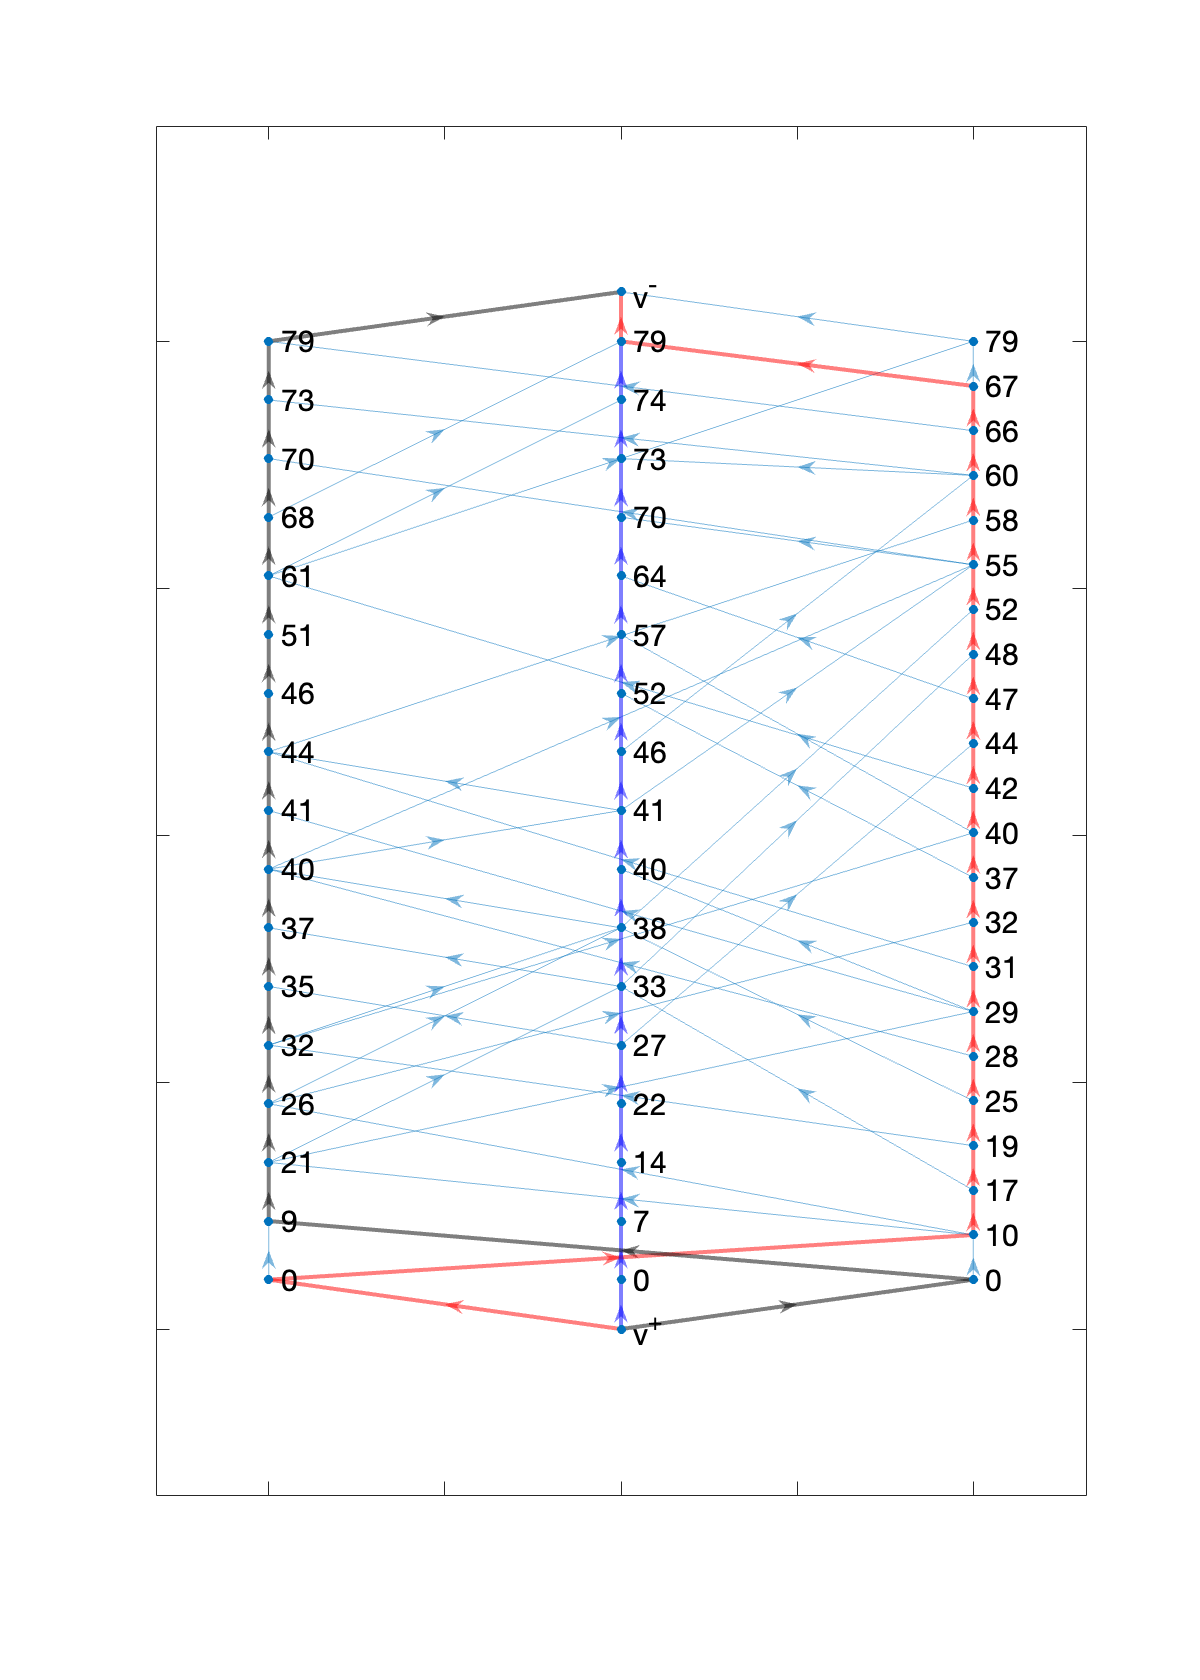
\includegraphics[width=0.4\linewidth]{graph_flow_result_3}
\caption{Security Graph and result for 3 flows}
\label{fig:security-graph-3-flow}
\end{center}
\end{figure}

\begin{figure}[htbp]
\begin{center}
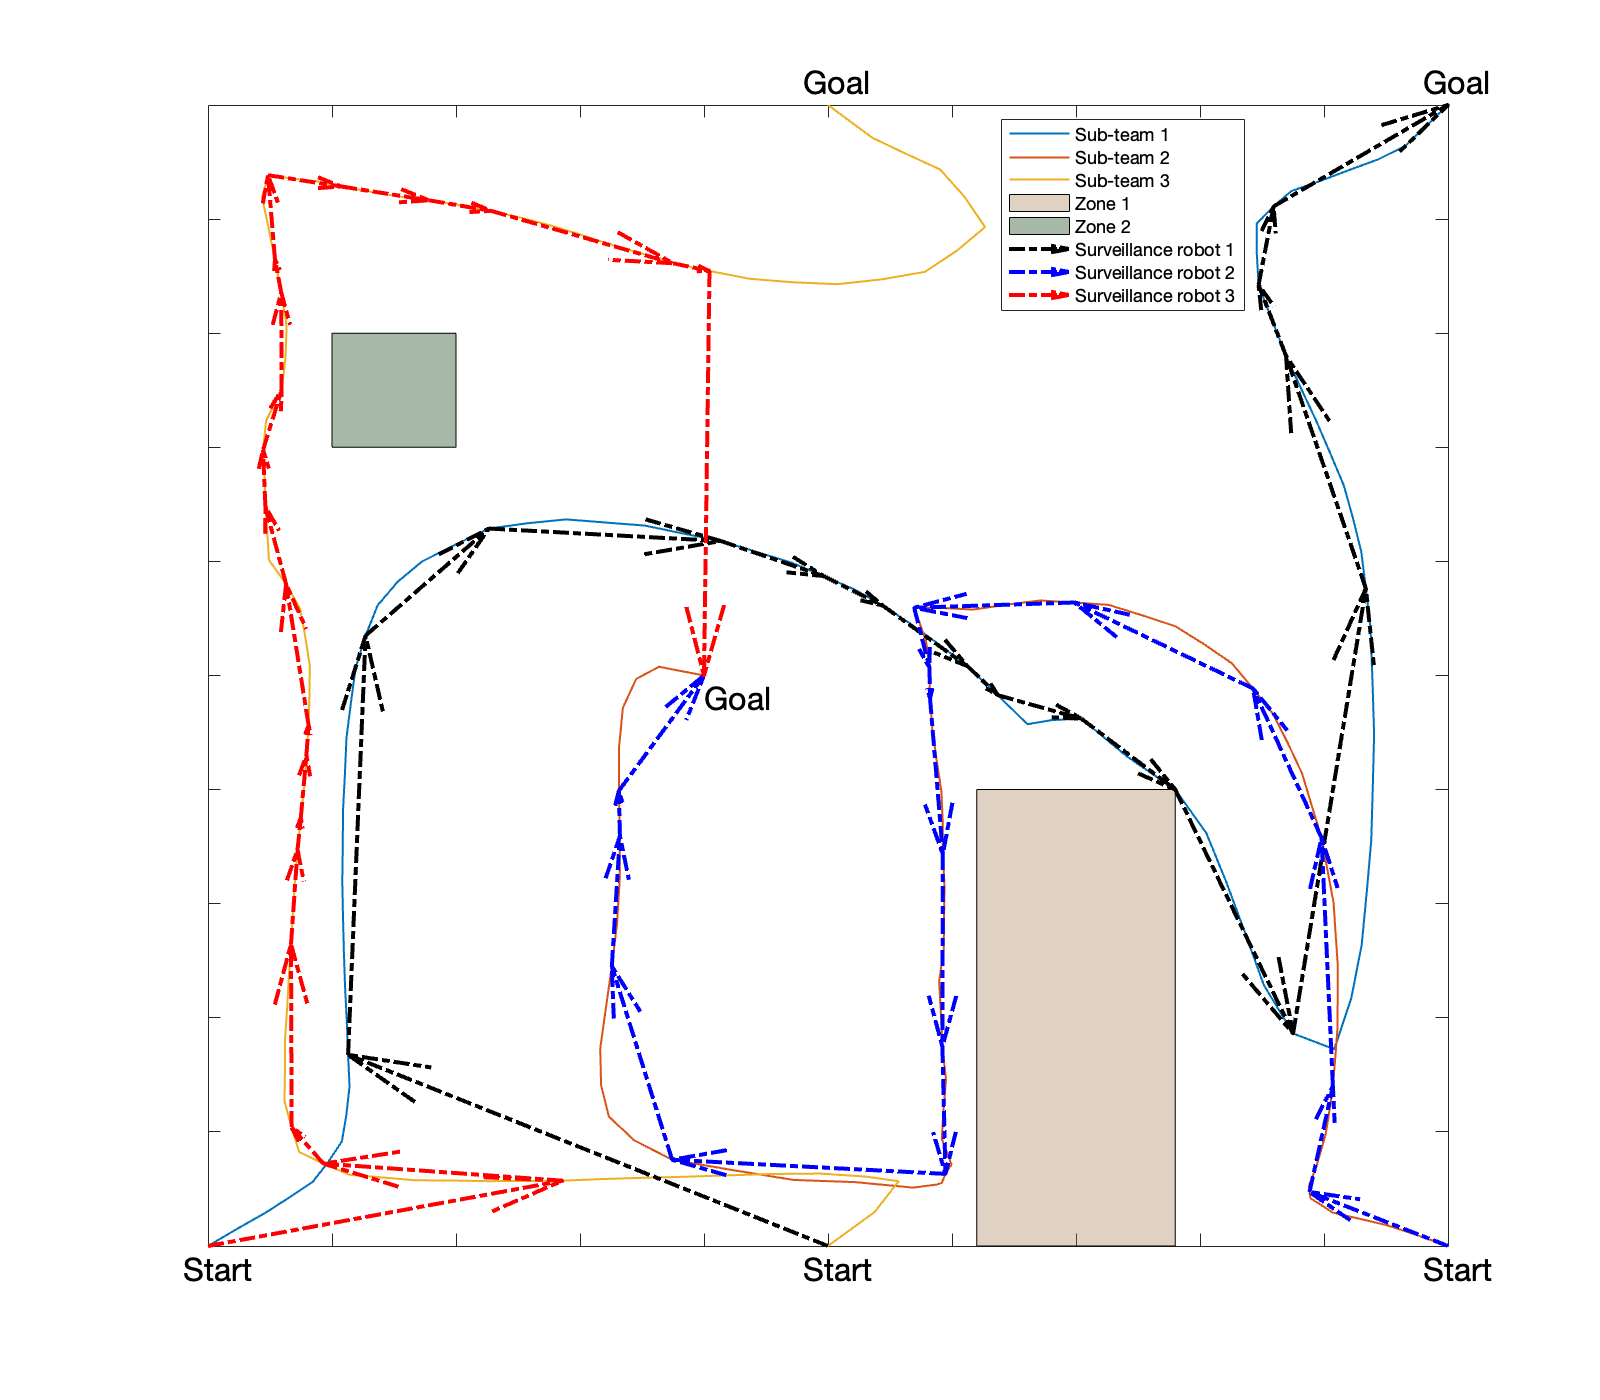
\includegraphics[width=0.6\linewidth]{3_flow_result}
\caption{Result of 3 surveillance agents' plan in workspace}
\label{fig:workspace-3-flow}
\end{center}
\end{figure}

We start by adding a total of $\cK=3$ surveillance robots into the workspace using the parameters $w_{c}=10$, $w_{t}=1$ and $\rho = 0.01$. The three trajectories are transformed into the graph $G$ shown in Figure \ref{fig:security-graph-3-flow}, where the number on each vertex $v_{i}$ represents the corresponding time $t_{i}$. Vertices in each column belong to the same trajectory, and edges across different columns are cross-trajectory edges. 

The flows derived from the solution of the optimization problem \eqref{eq:flow-coverage-problem} are highlighted in the graph. The planning result in the workspace is shown in \ref{fig:workspace-3-flow} as dash-dotted arrows with the same color used for each flow in \ref{fig:security-graph-3-flow}. Notice that flows represent the robot co-observation plan instead of actual robots, such that the red flow, for example, shows that the sub-team 2 is expecting a robot from sub-team 1, departing at $t=0$ and arriving at $t=10$, and needs to send a robot (not necessarily the same one received from sub-team 1) to sub-team 3, departing at $t=67$ and arriving at $t=79$. This plan is not ideal in terms of our security criteria since co-observations happens between the same pair of surveillance robot and sub-team for the majority of the time with only three cross-trajectory edges that are covered.

\begin{figure}[t]
\begin{center}
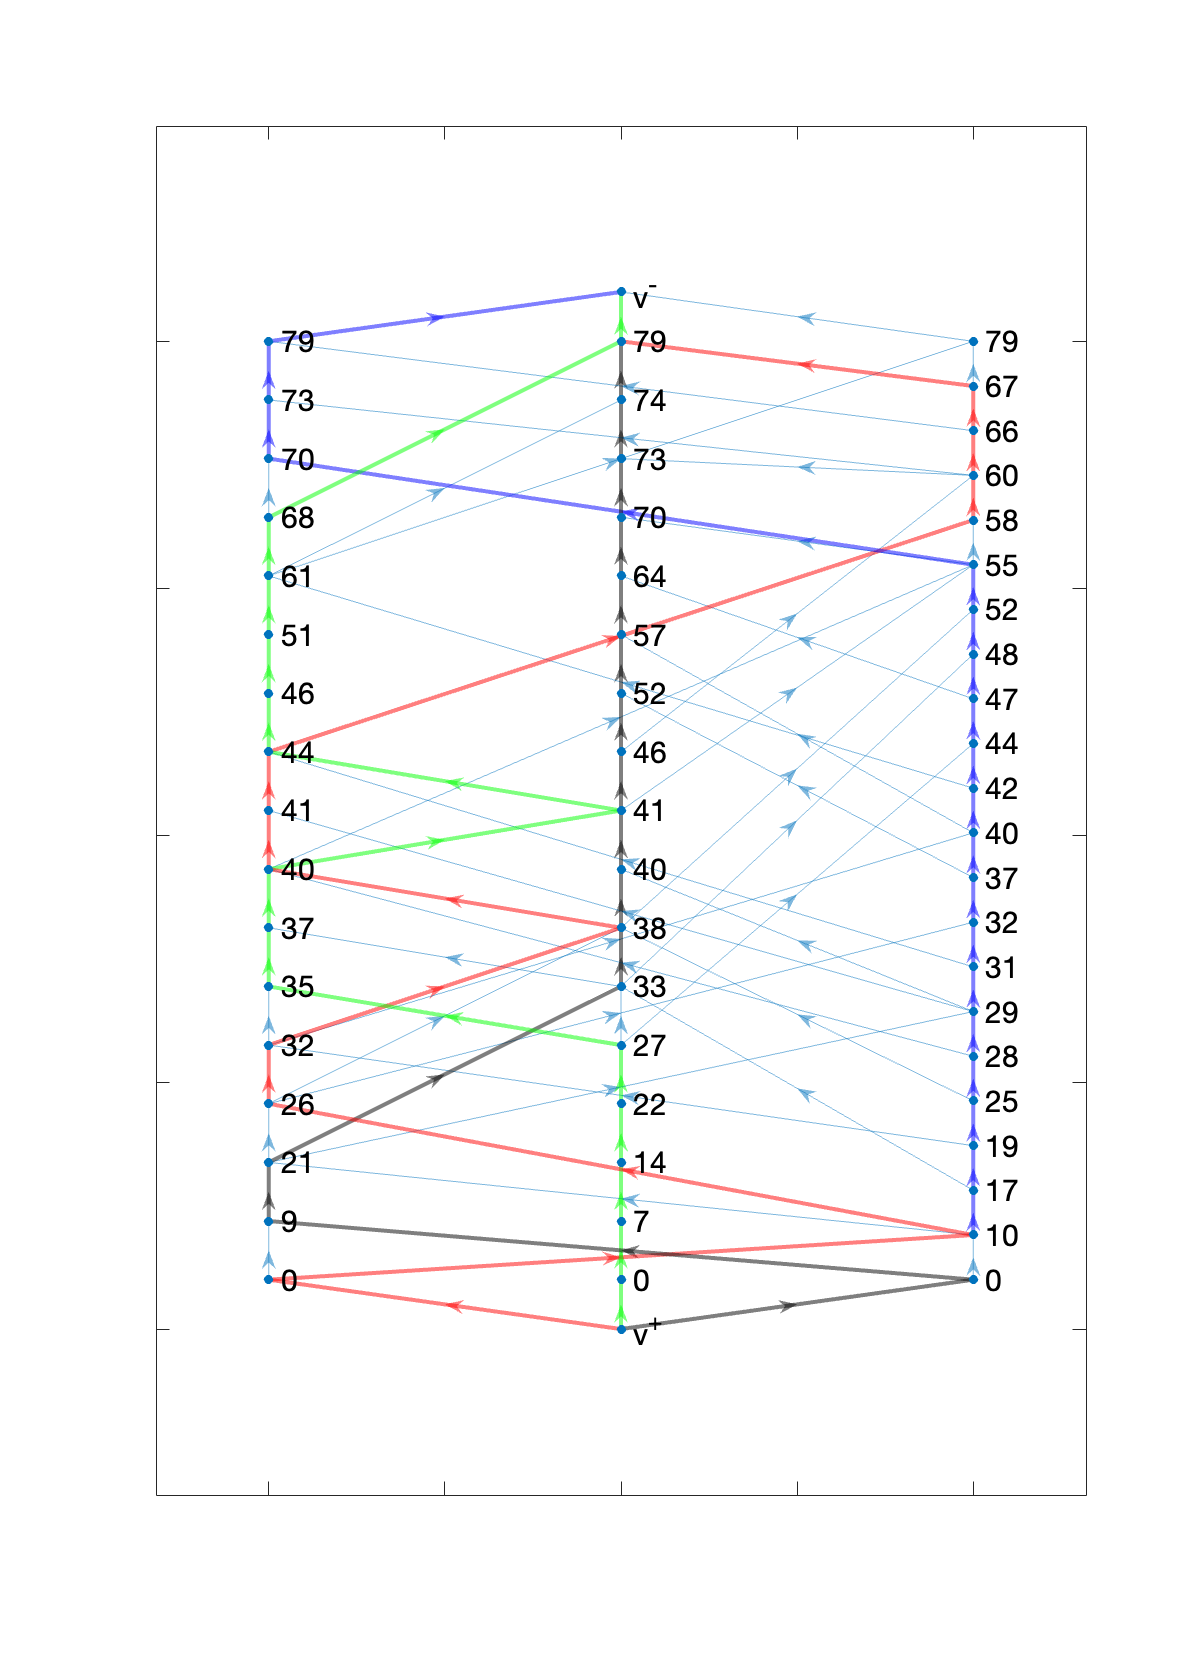
\includegraphics[width=0.4\linewidth]{graph_flow_result_4}
\caption{Security Graph and result for 4 flows.}
\label{fig:security-graph-4-flow}
\end{center}
\end{figure}

\begin{figure}[htbp]
\begin{center}
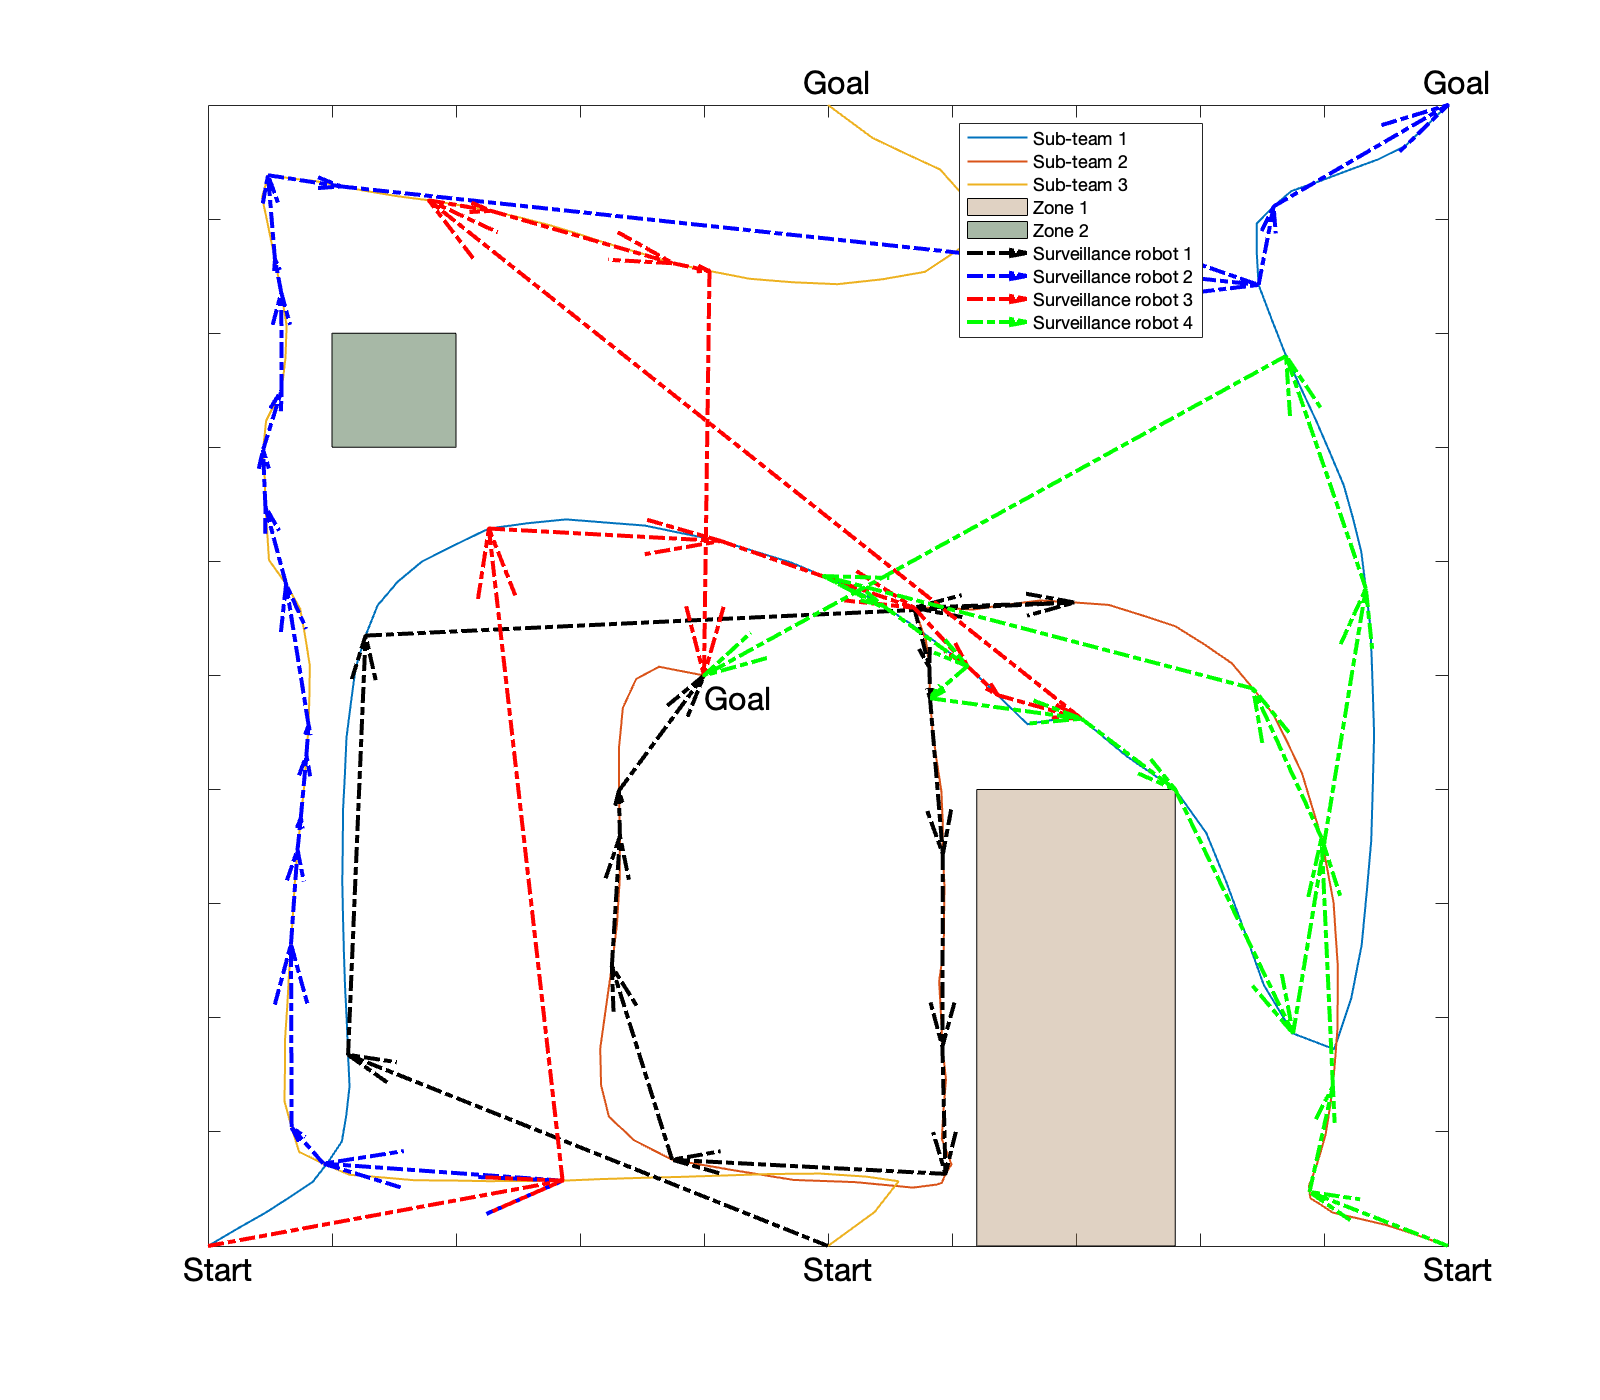
\includegraphics[width=0.6\linewidth]{4_flow_result}
\caption{Result of 3 surveillance agents' plan in work space.}
\label{fig:workspace-4-flow}
\end{center}
\end{figure}

For the case where $\cK=4$, the results are shown in Figure \ref{fig:security-graph-4-flow}-\ref{fig:workspace-4-flow}. With one additional robot added, there are significant increase in the total cross-trajectory edges covered, and sub-teams performs co-observation with different robots during the task period.

If we further increase $\cK>4$, we do not get a better result; instead, the planner will generate 4 flows with the rest $\cK-4$ flows empty.

\begin{figure}[htbp]
\begin{center}
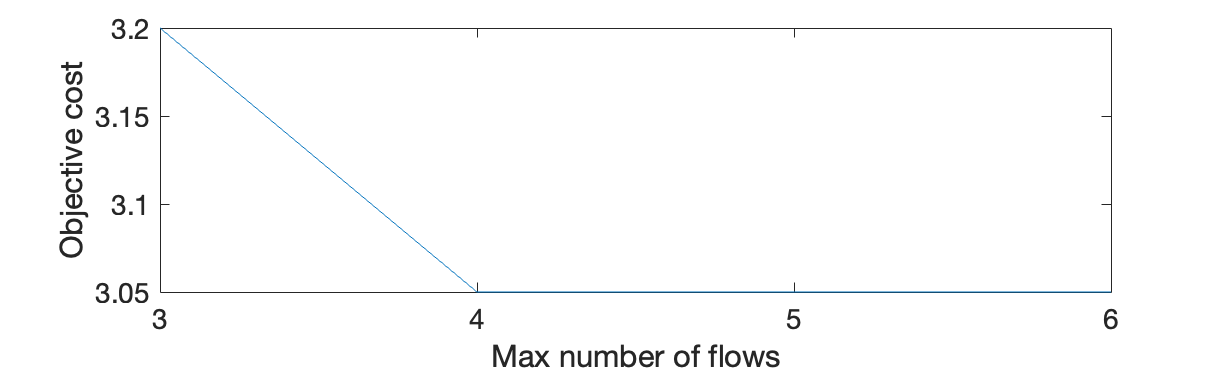
\includegraphics[width=0.6\linewidth]{nflow_vs_cost}
\caption{Plan reach optimality when $\cK=4$, further increase of $\cK$ does not increase the cost of objectives.}
\label{fig:flow-n-vs-cost}
\end{center}
\end{figure}

\section{Summary}
In this chapter, we provide a method to enhance the security of a multi-robot system without sacrificing the performance. This is done by introducing additional robots to perform cross-trajectory co-observations by traveling between different trajectories. We model the unsecured multi-robot trajectories as a checkpoint graph by identifying checkpoints that requires observation and cross-trajectory paths that can safely access the checkpoints from different trajectories. We have shown that the co-observation planning problem across different trajectories can be transformed into a multi flow problem on the graph, and that we can find the minimal number of robot needed to finish the co-observation task.



{\small
\bibliographystyle{unsrt}
\bibliography{ADMM_planning,ACC}
}

\end{document}
